\input{preamble}

\begin{document}

\begin{flushright}
Laura Fields\\
Paul Lebrun \\
Seongtae Park \\
Add more here \\
\today
\end{flushright}

%title
\begin{center}

{\LARGE LBNE Beam Alignment Tolerances}
\end{center}

%\tableofcontents

%\begin{abstract} 	

%\end{abstract}
\section{Introduction}

This note describes a study of LBNE beamline alignment tolerances and systematic uncertainties that was conducted in the winter of 2013-2014.  For each major source of beamline systematic uncertainty (listed in Table~\ref{tab:syslist}), we evaluate the systematic uncertainty on the flux at the nominal tolerance (also listed in Table~\ref{tab:syslist}, obtained from the LBNE CDR ~\cite{lbnecdr} where applicable and from consulation with beamline experts otherwise).  

\section{Description of Beam Simulation|

\section{Procedure for Evaluating Systematic Uncertainties}
\label{sec:procedure}

In all cases, we evaluate the uncertainty on the flux at the near detector, at the far detector and on the near/far flux ratio between zero and 10 GeV in bins of 0.5 GeV.  Section~\ref{sec:procedure}

\section{Conclusions}

\appendix
\section{Flux Variation and Fit Plots}

\vspace{3in}


\begin{figure}[ht]
  \begin{center}
    {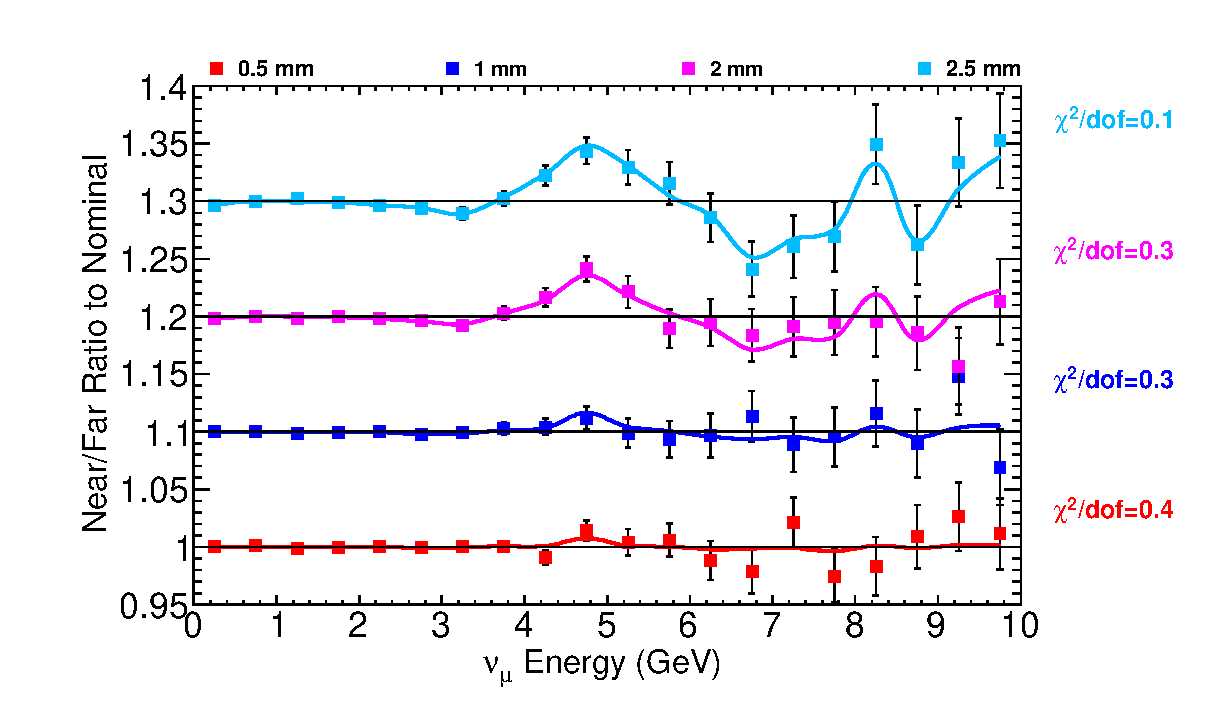
\includegraphics[width=6.0in]{figures/Horn1XOffset_nof_summary.eps}}
  \end{center}
\caption{ Near/Far double ratios to nominal for several values of {\bf Horn 1 Offset in $x$} (points) and the results of the fits to each energy bin (lines).}
\end{figure}

\begin{figure}[ht]
  \begin{center}
    {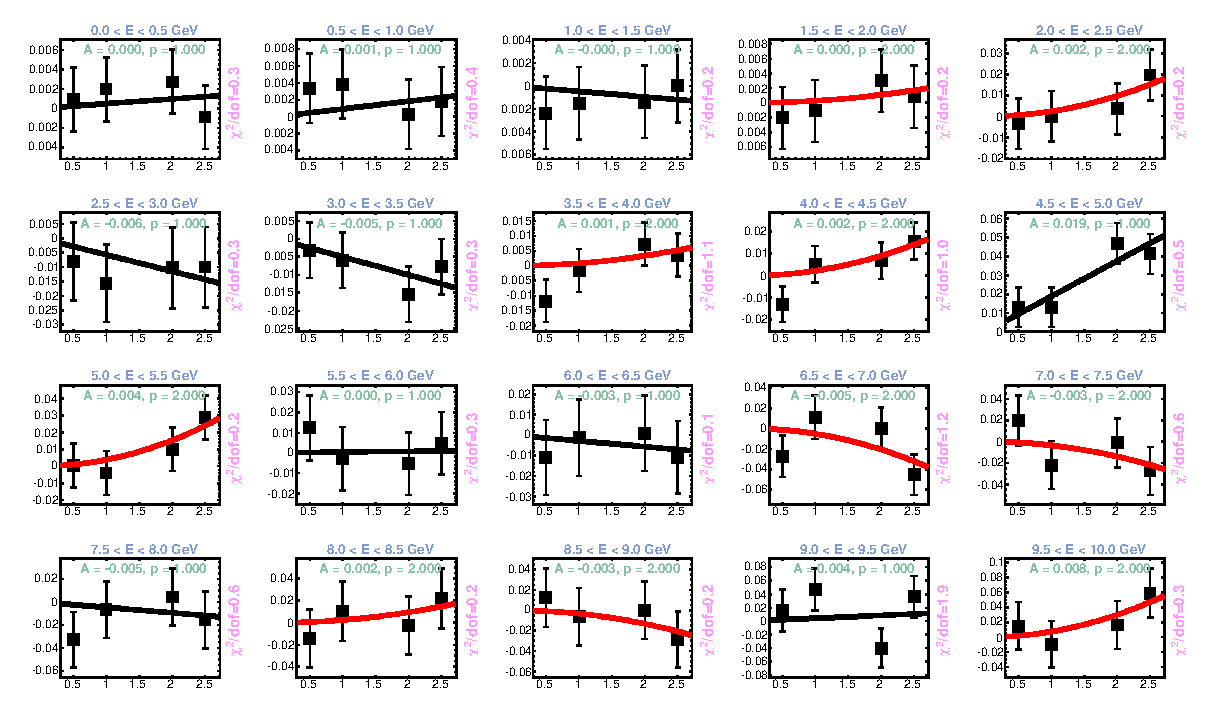
\includegraphics[width=5.0in]{figures/Horn1XOffset_nof_fits.eps}}
  \end{center}
\caption{ Fits to the near/far ratios for several values of {\bf Horn 1 Offset in $x$}. Black(Red) fit lines indicate that a linear(parabolic) fit provided the best $\chi^2$. }
\end{figure}

\begin{figure}[ht]
  \begin{center}
    {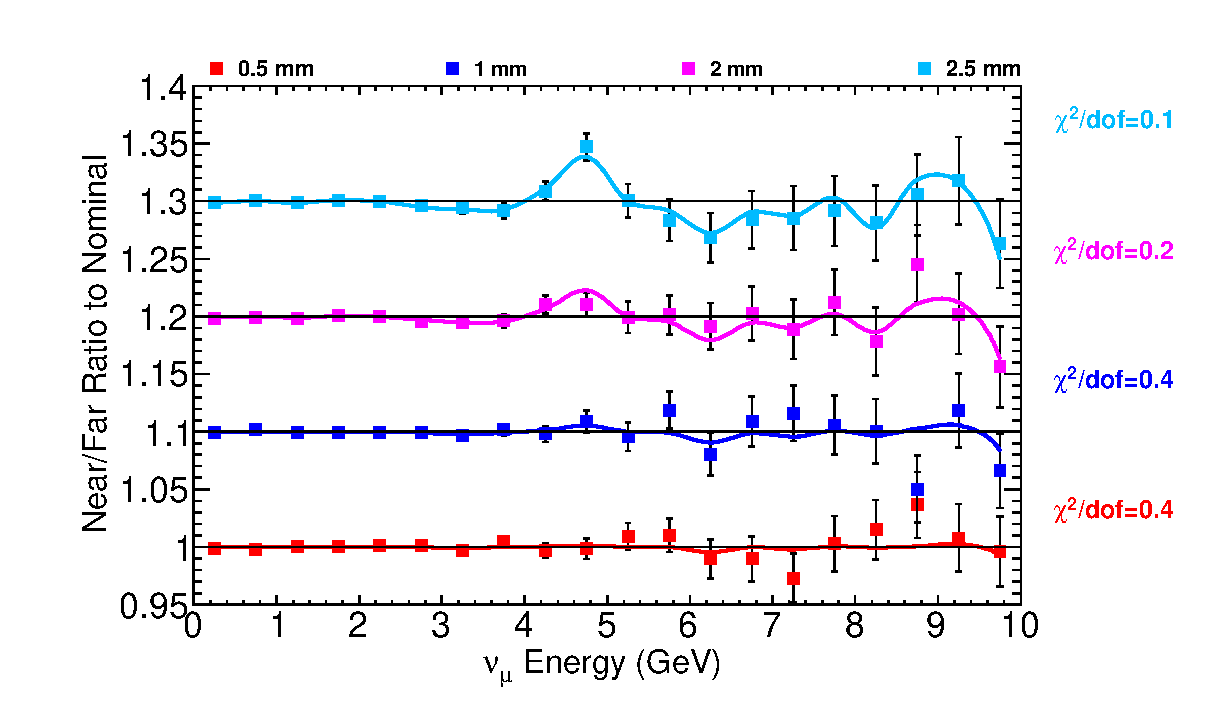
\includegraphics[width=6.0in]{figures/Horn1YOffset_nof_summary.eps}}
  \end{center}
\caption{ Near/Far double ratios to nominal for several values of {\bf Horn 1 Offset in $y$} (points) and the results of the fits to each energy bin (lines).}
\end{figure}

\begin{figure}[ht]
  \begin{center}
    {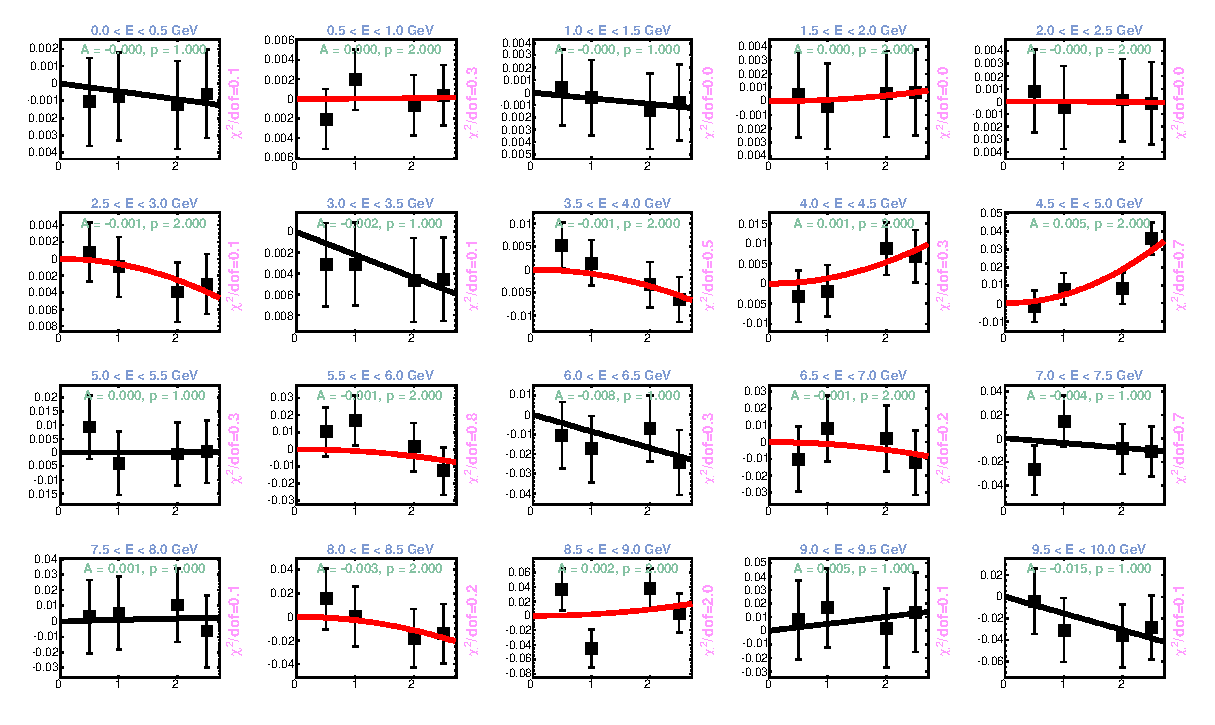
\includegraphics[width=5.0in]{figures/Horn1YOffset_nof_fits.eps}}
  \end{center}
\caption{ Fits to the near/far ratios for several values of {\bf Horn 1 Offset in $y$}. Black(Red) fit lines indicate that a linear(parabolic) fit provided the best $\chi^2$. }
\end{figure}

\begin{figure}[ht]
  \begin{center}
    {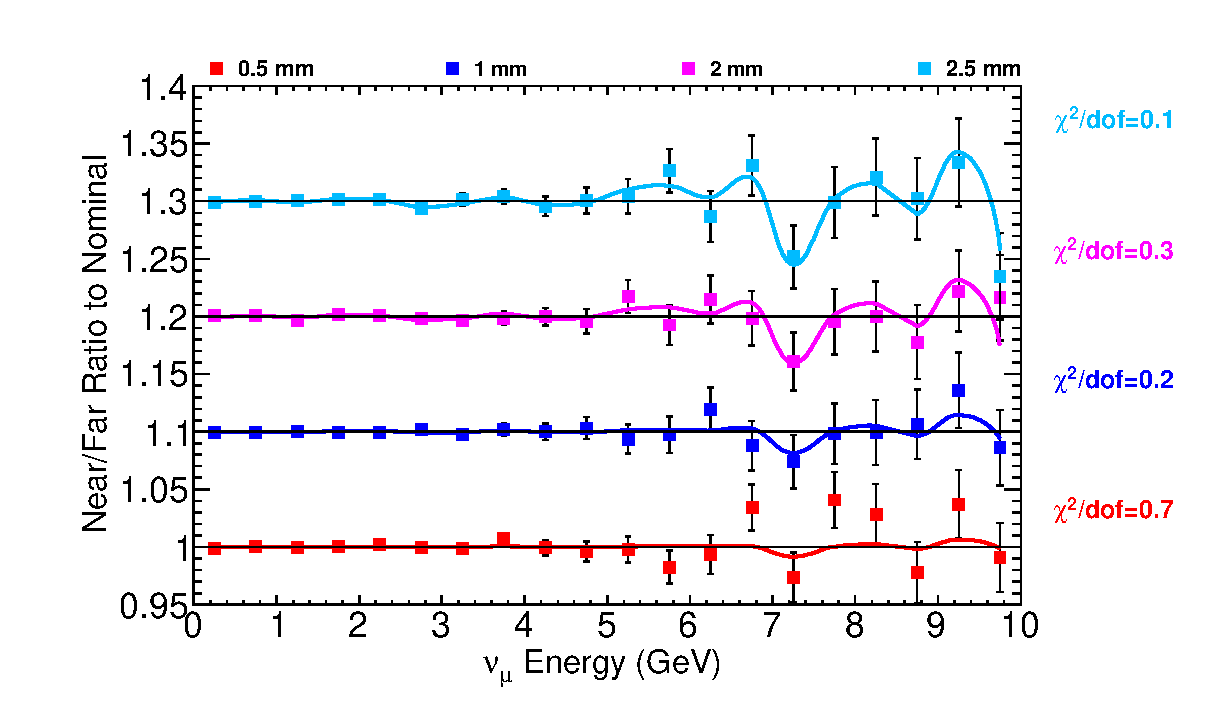
\includegraphics[width=6.0in]{figures/Horn2XOffset_nof_summary.eps}}
  \end{center}
\caption{ Near/Far double ratios to nominal for several values of {\bf Horn 2 Offset in $x$} (points) and the results of the fits to each energy bin (lines).}
\end{figure}

\begin{figure}[ht]
  \begin{center}
    {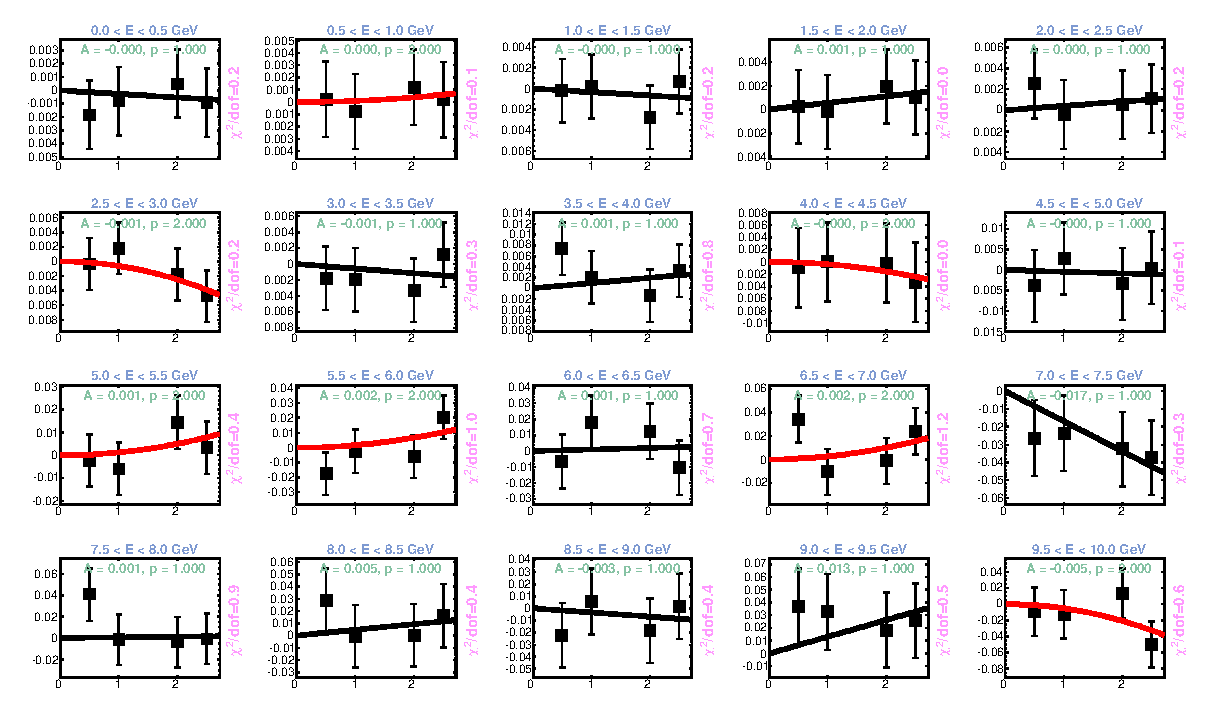
\includegraphics[width=5.0in]{figures/Horn2XOffset_nof_fits.eps}}
  \end{center}
\caption{ Fits to the near/far ratios for several values of {\bf Horn 2 Offset in $x$}. Black(Red) fit lines indicate that a linear(parabolic) fit provided the best $\chi^2$. }
\end{figure}

\begin{figure}[ht]
  \begin{center}
    {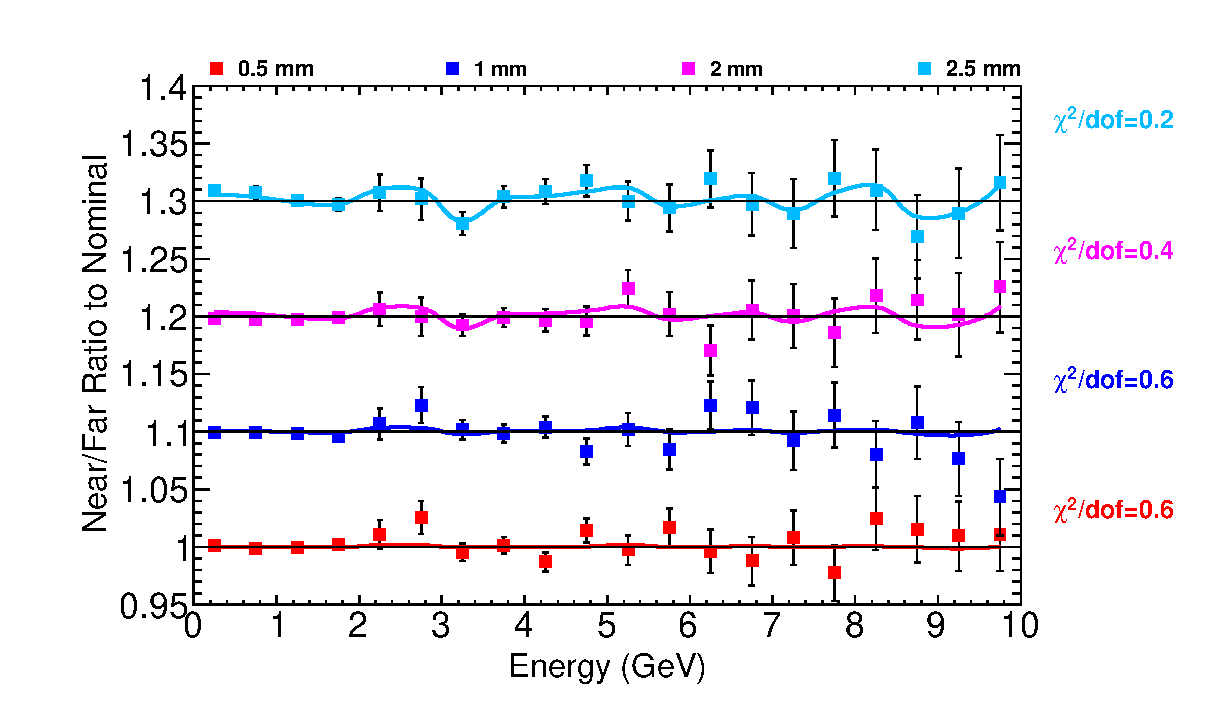
\includegraphics[width=6.0in]{figures/Horn2YOffset_nof_summary.eps}}
  \end{center}
\caption{ Near/Far double ratios to nominal for several values of {\bf Horn 2 Offset in $y$} (points) and the results of the fits to each energy bin (lines).}
\end{figure}

\begin{figure}[ht]
  \begin{center}
    {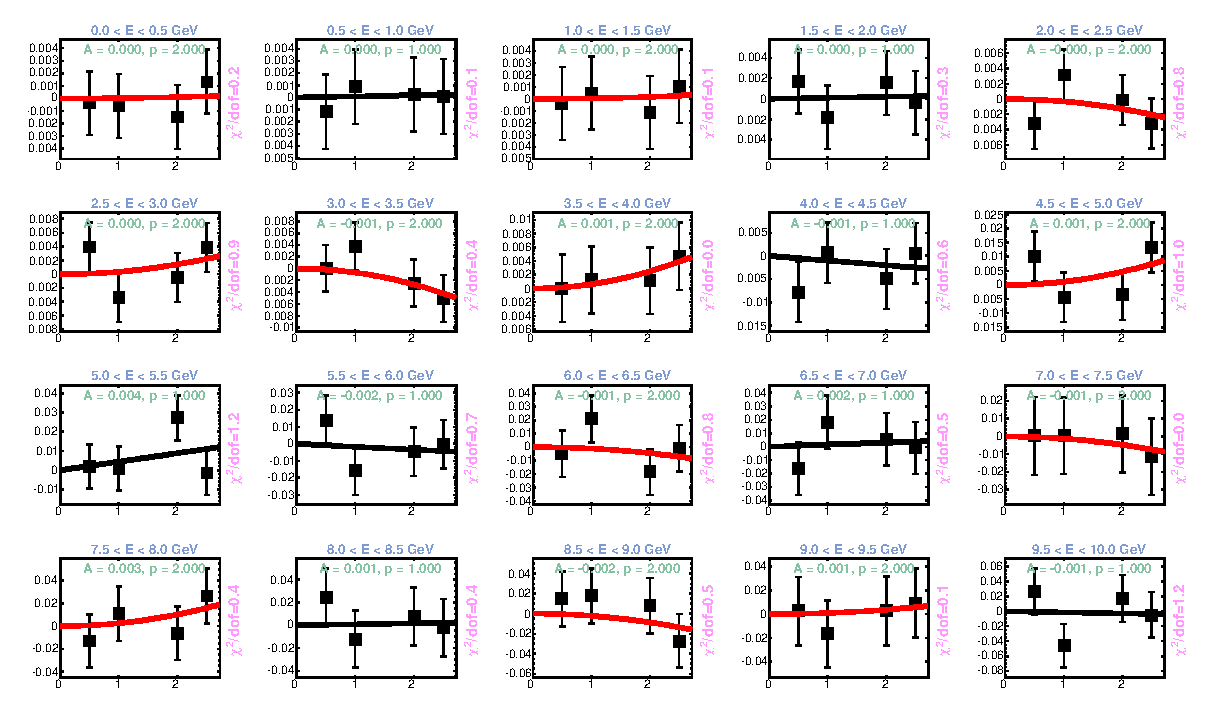
\includegraphics[width=5.0in]{figures/Horn2YOffset_nof_fits.eps}}
  \end{center}
\caption{ Fits to the near/far ratios for several values of {\bf Horn 2 Offset in $y$}. Black(Red) fit lines indicate that a linear(parabolic) fit provided the best $\chi^2$. }
\end{figure}

\begin{figure}[ht]
  \begin{center}
    {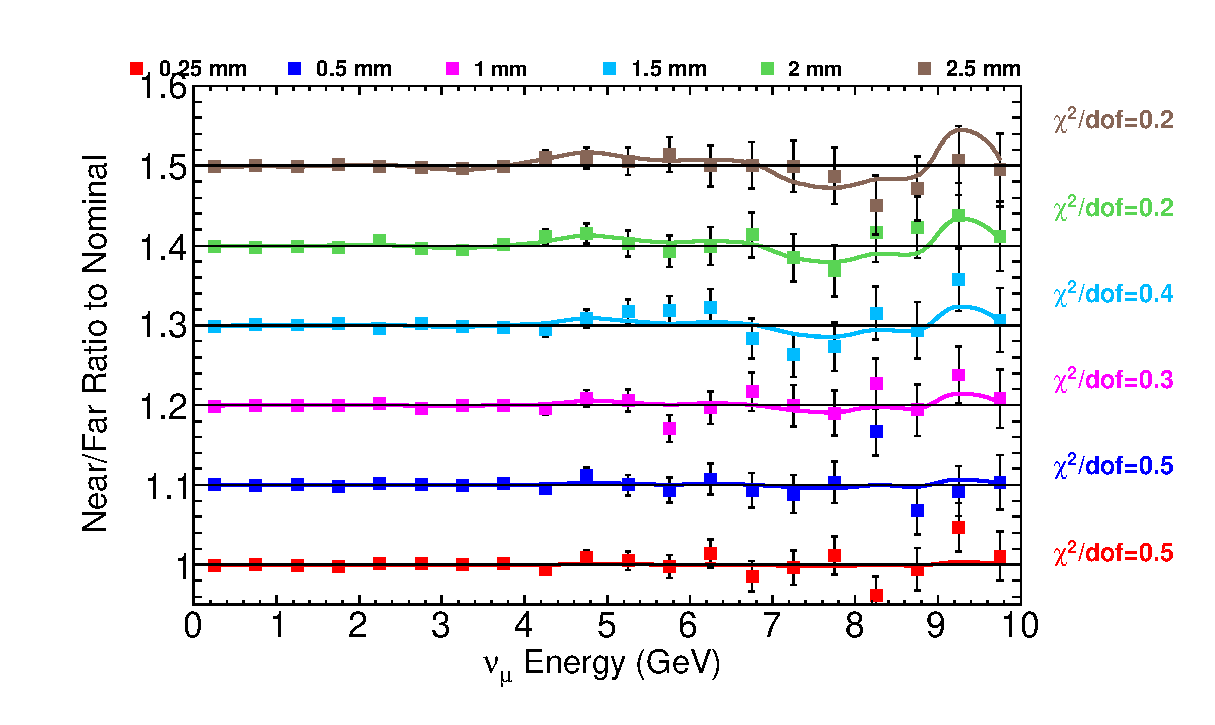
\includegraphics[width=6.0in]{figures/Horn1XTilt_nof_summary.eps}}
  \end{center}
\caption{ Near/Far double ratios to nominal for several values of {\bf Horn 1 Tilt in $x$} (points) and the results of the fits to each energy bin (lines).}
\end{figure}

\begin{figure}[ht]
  \begin{center}
    {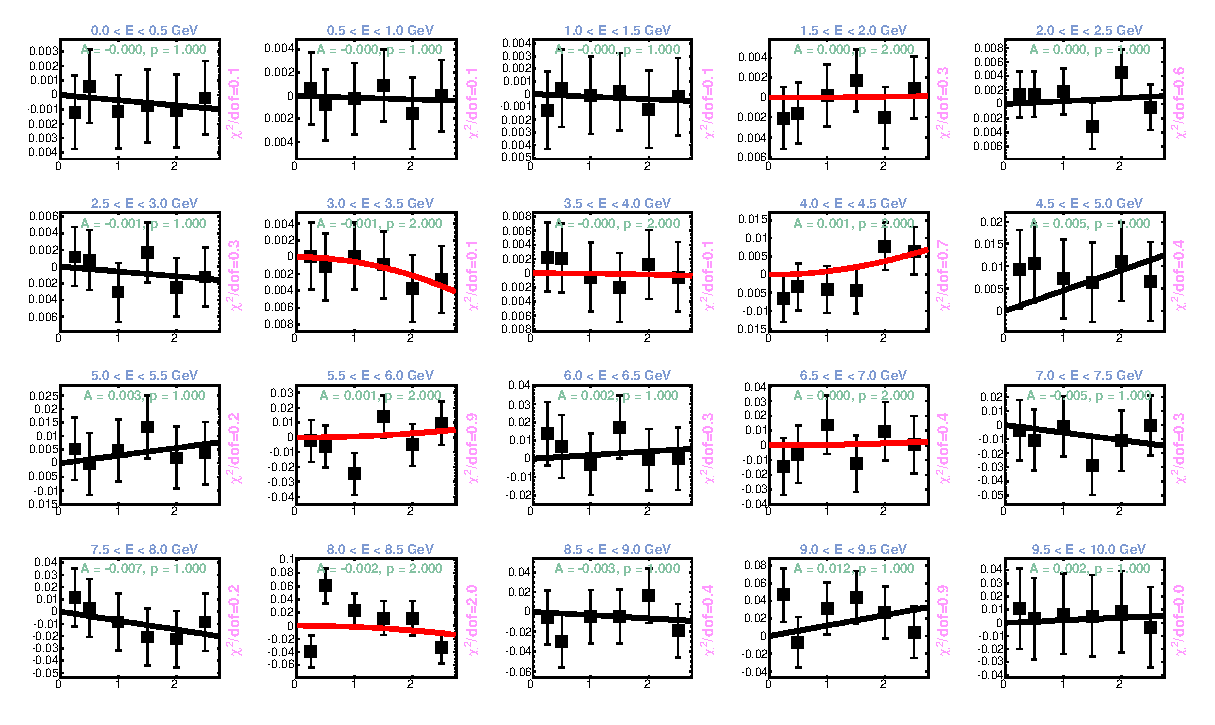
\includegraphics[width=5.0in]{figures/Horn1XTilt_nof_fits.eps}}
  \end{center}
\caption{ Fits to the near/far ratios for several values of {\bf Horn 1 Tilt in $x$}. Black(Red) fit lines indicate that a linear(parabolic) fit provided the best $\chi^2$. }
\end{figure}

\begin{figure}[ht]
  \begin{center}
    {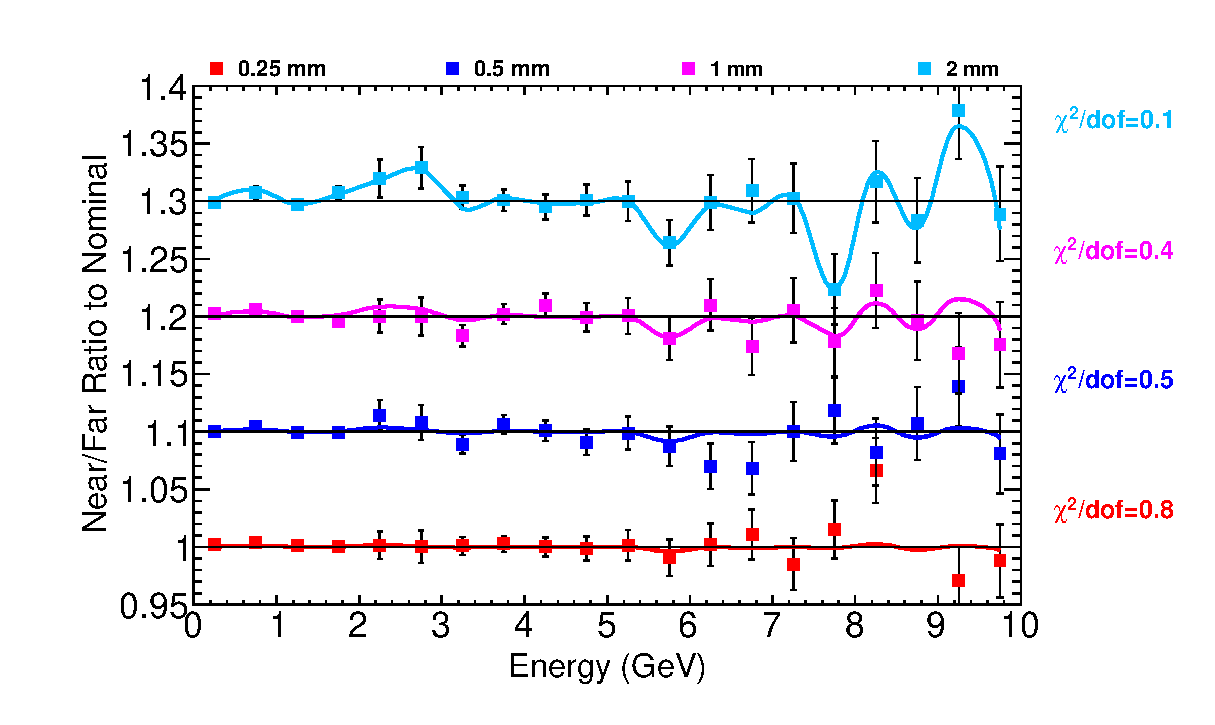
\includegraphics[width=6.0in]{figures/Horn1YTilt_nof_summary.eps}}
  \end{center}
\caption{ Near/Far double ratios to nominal for several values of {\bf Horn 1 Tilt in $y$} (points) and the results of the fits to each energy bin (lines).}
\end{figure}

\clearpage

\begin{figure}[ht]
  \begin{center}
    {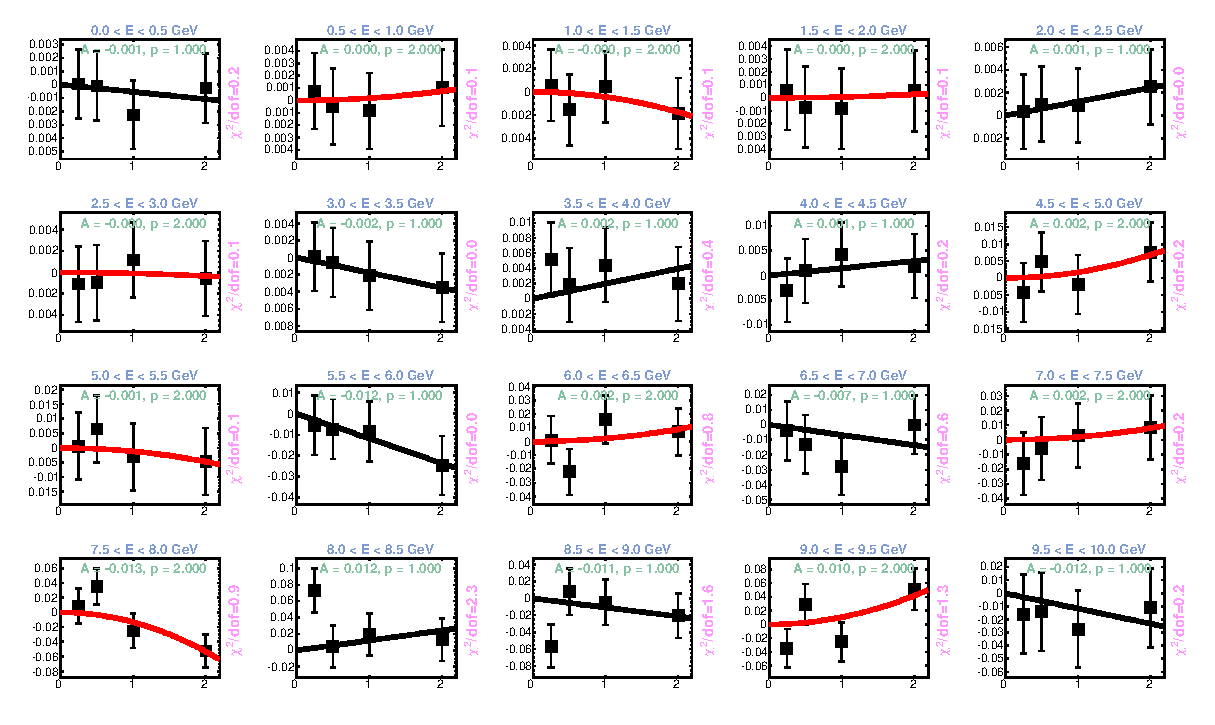
\includegraphics[width=5.0in]{figures/Horn1YTilt_nof_fits.eps}}
  \end{center}
\caption{ Fits to the near/far ratios for several values of {\bf Horn 1 Tilt in $y$}. Black(Red) fit lines indicate that a linear(parabolic) fit provided the best $\chi^2$. }
\end{figure}



\begin{figure}[ht]
  \begin{center}
    {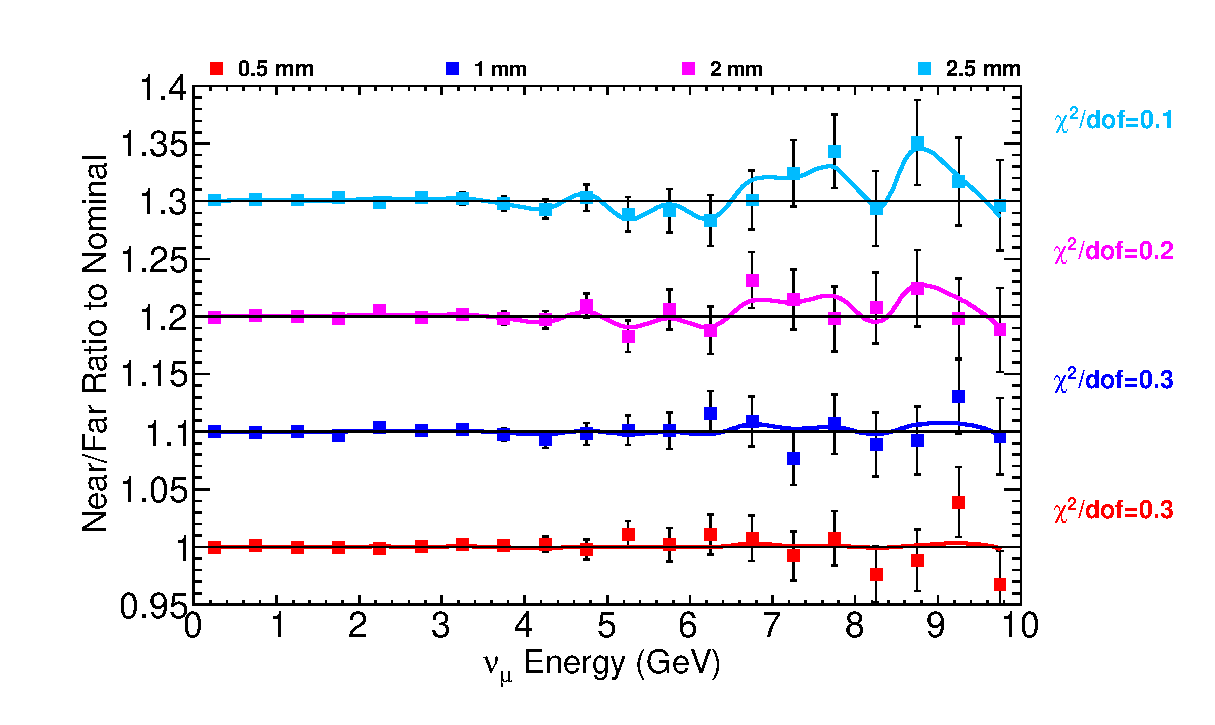
\includegraphics[width=6.0in]{figures/Horn2XTilt_nof_summary.eps}}
  \end{center}
\caption{ Near/Far double ratios to nominal for several values of {\bf Horn 2 Tilt in $x$} (points) and the results of the fits to each energy bin (lines).}
\end{figure}

\begin{figure}[ht]
  \begin{center}
    {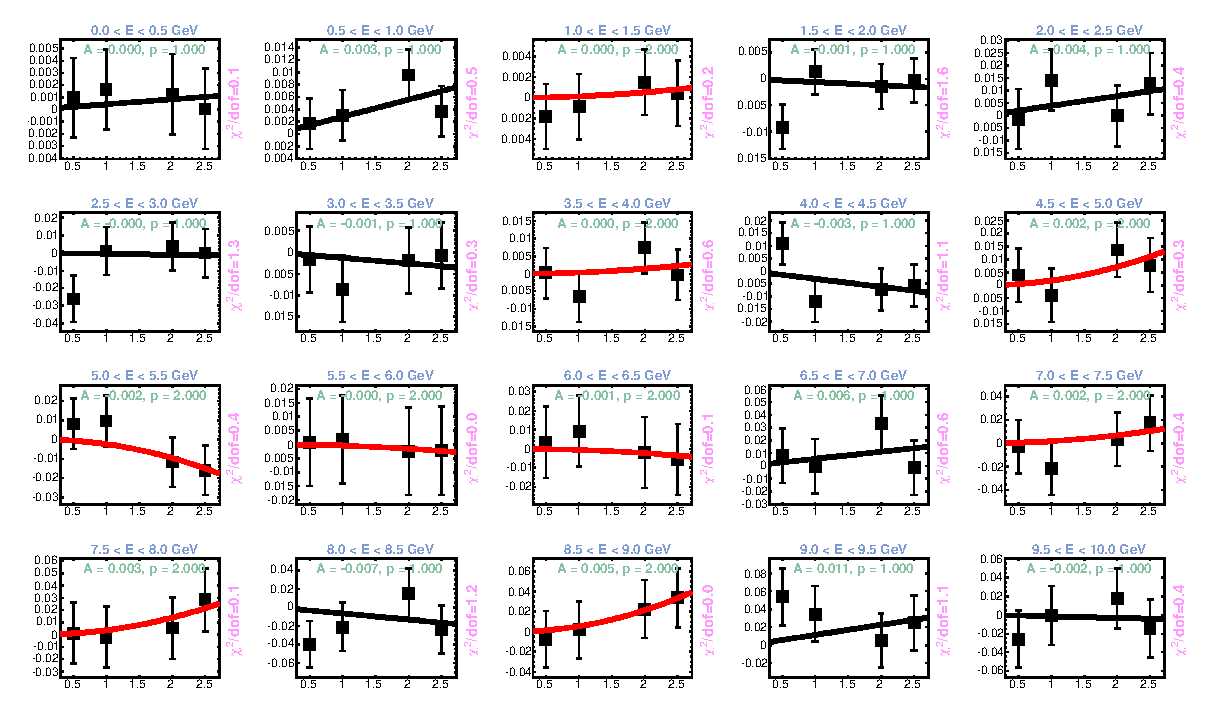
\includegraphics[width=5.0in]{figures/Horn2XTilt_nof_fits.eps}}
  \end{center}
\caption{ Fits to the near/far ratios for several values of {\bf Horn 2 Tilt in $x$}. Black(Red) fit lines indicate that a linear(parabolic) fit provided the best $\chi^2$. }
\end{figure}

\begin{figure}[ht]
  \begin{center}
    {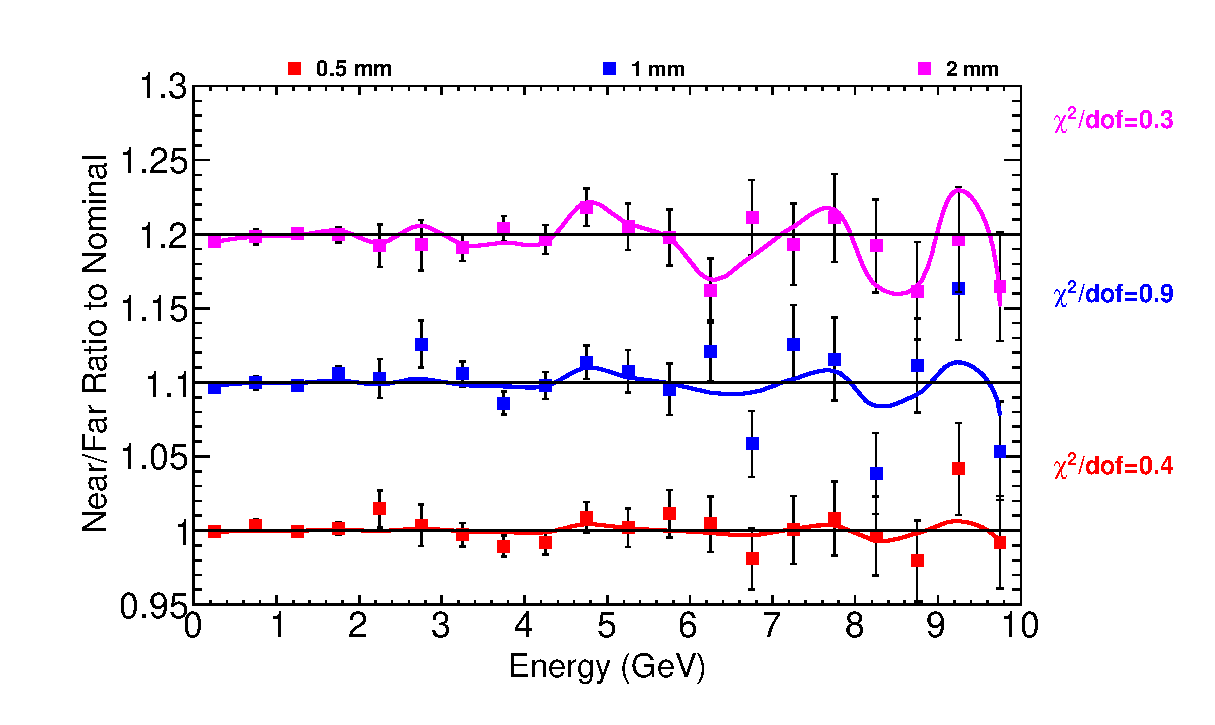
\includegraphics[width=6.0in]{figures/Horn2YTilt_nof_summary.eps}}
  \end{center}
\caption{ Near/Far double ratios to nominal for several values of {\bf Horn 2 Tilt in $y$} (points) and the results of the fits to each energy bin (lines).}
\end{figure}

\begin{figure}[ht]
  \begin{center}
    {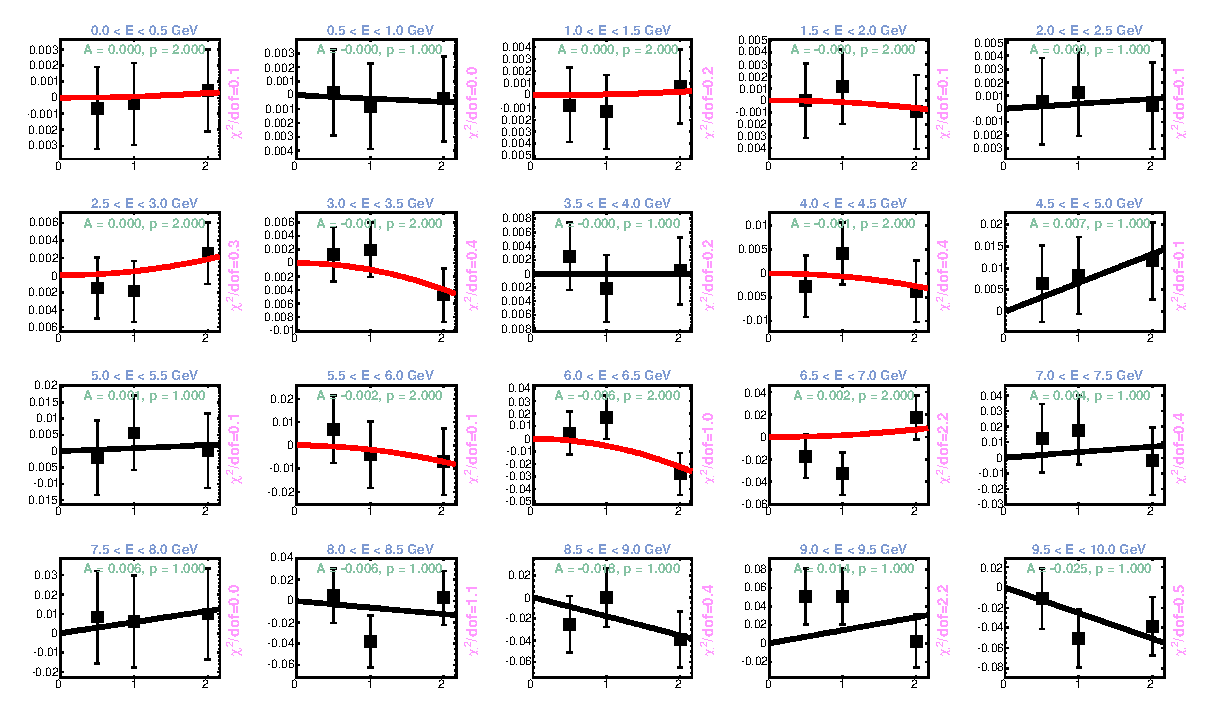
\includegraphics[width=5.0in]{figures/Horn2YTilt_nof_fits.eps}}
  \end{center}
\caption{ Fits to the near/far ratios for several values of {\bf Horn 2 Tilt in $y$}. Black(Red) fit lines indicate that a linear(parabolic) fit provided the best $\chi^2$. }
\end{figure}

\begin{figure}[ht]
  \begin{center}
    {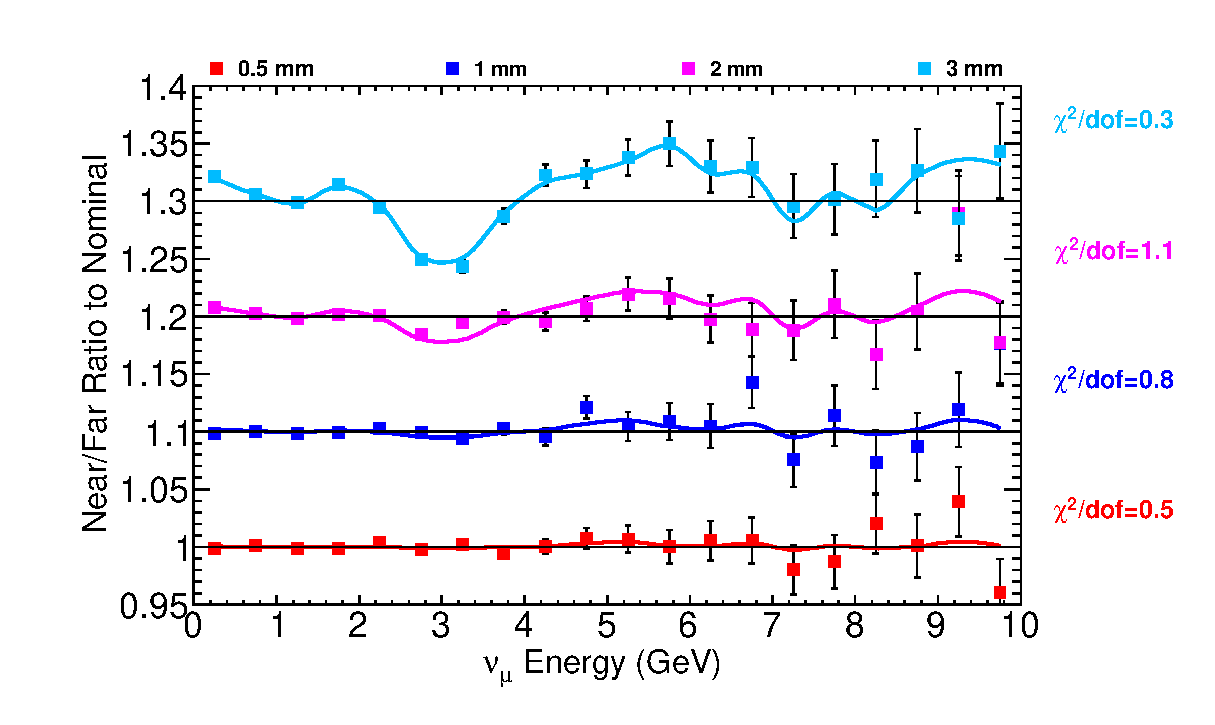
\includegraphics[width=6.0in]{figures/TargetXOffset_nof_summary.eps}}
  \end{center}
\caption{ Near/Far double ratios to nominal for several values of {\bf Target Offset in $x$} (points) and the results of the fits to each energy bin (lines).}
\end{figure}

\begin{figure}[ht]
  \begin{center}
    {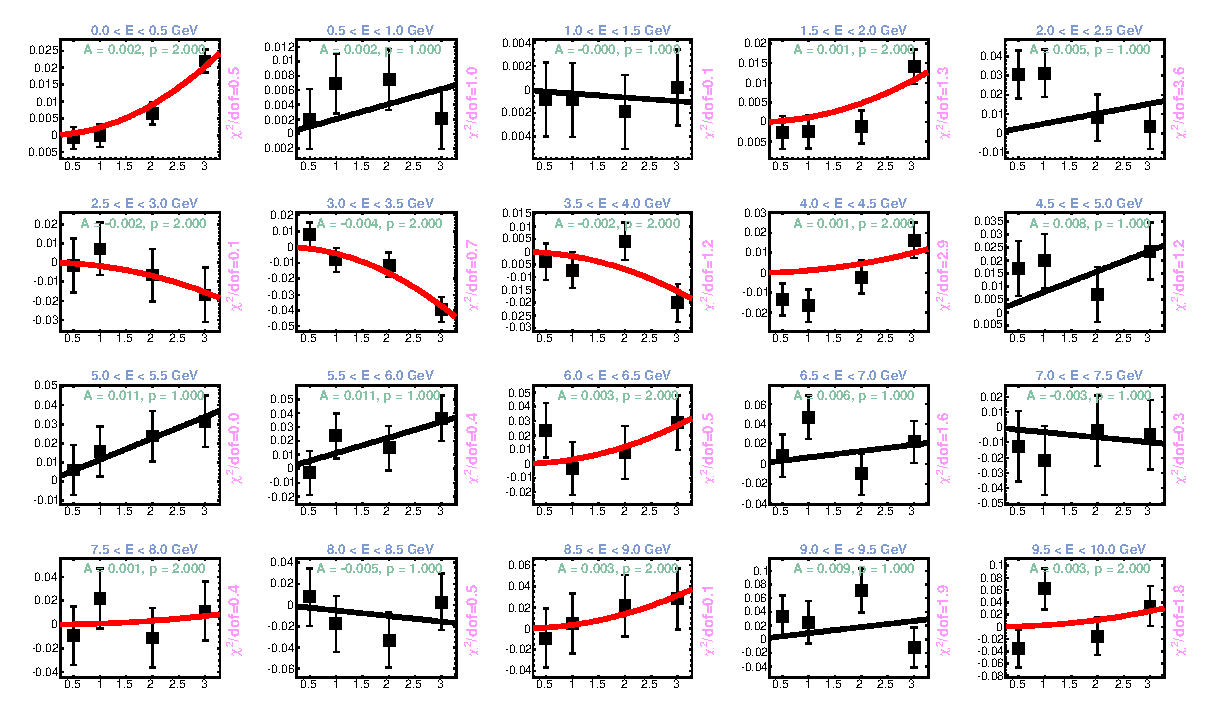
\includegraphics[width=5.0in]{figures/TargetXOffset_nof_fits.eps}}
  \end{center}
\caption{ Fits to the near/far ratios for several values of {\bf Target Offset in $x$}. Black(Red) fit lines indicate that a linear(parabolic) fit provided the best $\chi^2$. }
\end{figure}

\begin{figure}[ht]
  \begin{center}
    {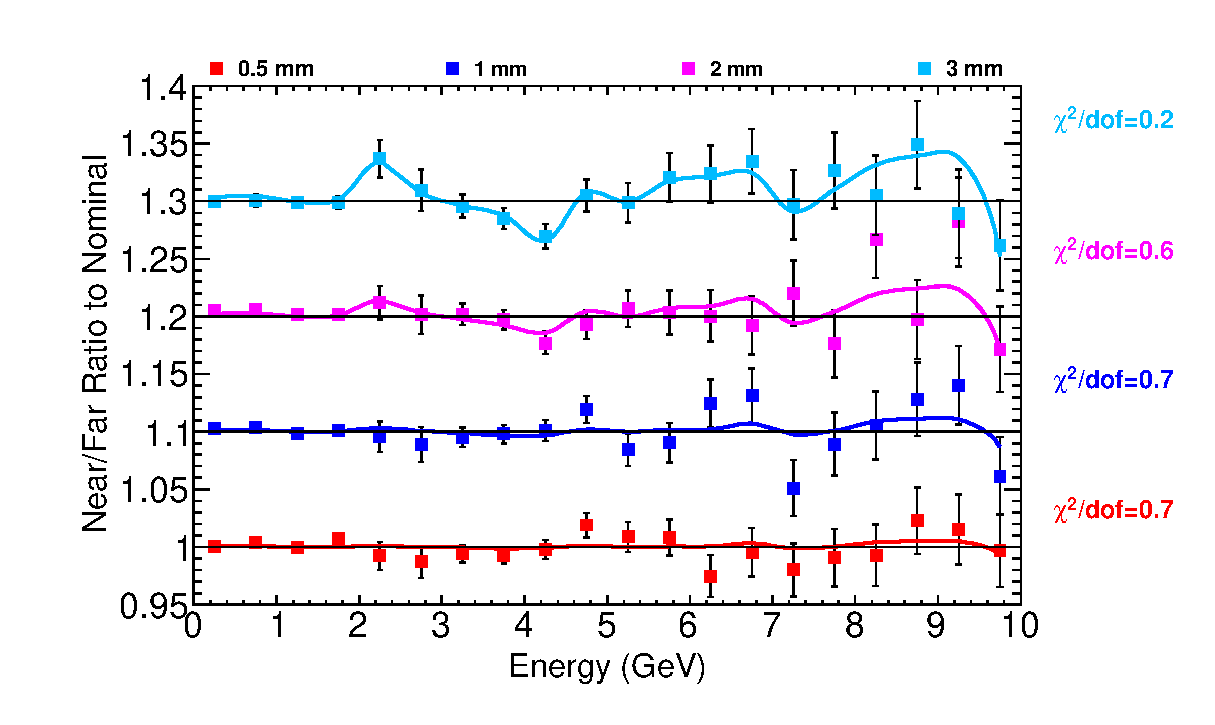
\includegraphics[width=6.0in]{figures/TargetYOffset_nof_summary.eps}}
  \end{center}
\caption{ Near/Far double ratios to nominal for several values of {\bf Target Offset in $y$} (points) and the results of the fits to each energy bin (lines).}
\end{figure}

\begin{figure}[ht]
  \begin{center}
    {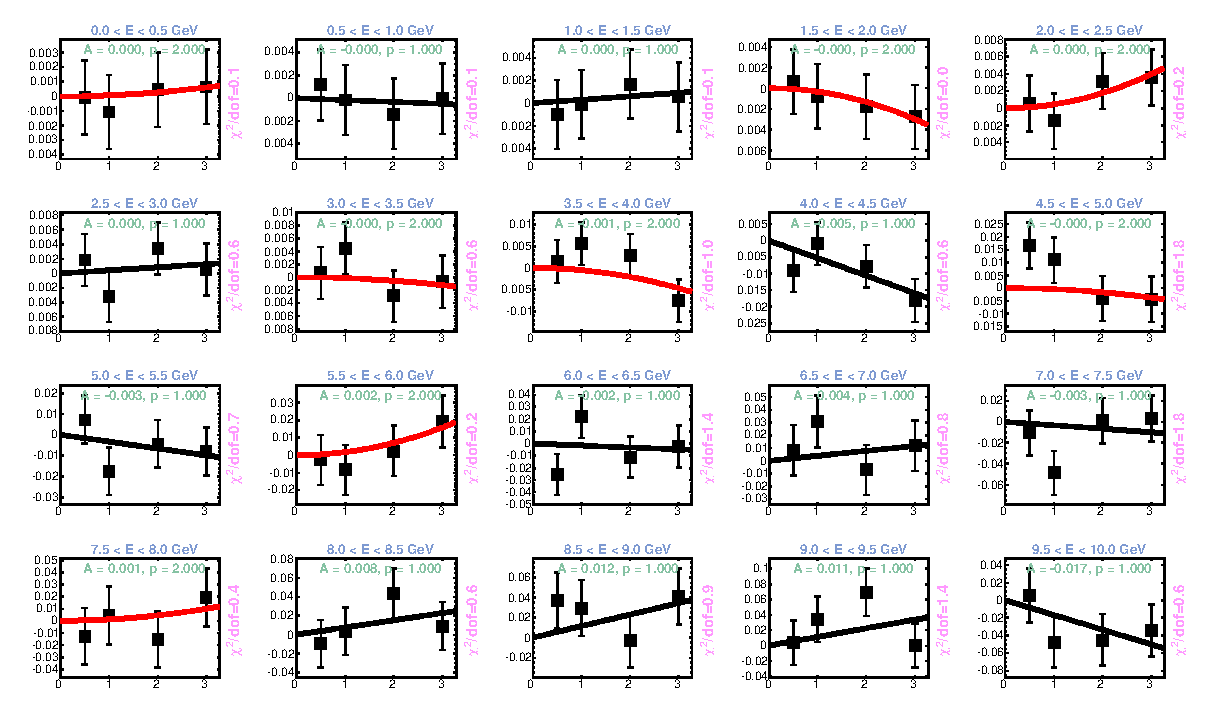
\includegraphics[width=5.0in]{figures/TargetYOffset_nof_fits.eps}}
  \end{center}
\caption{ Fits to the near/far ratios for several values of {\bf Target Offset in $y$}. Black(Red) fit lines indicate that a linear(parabolic) fit provided the best $\chi^2$. }
\end{figure}

\begin{figure}[ht]
  \begin{center}
    {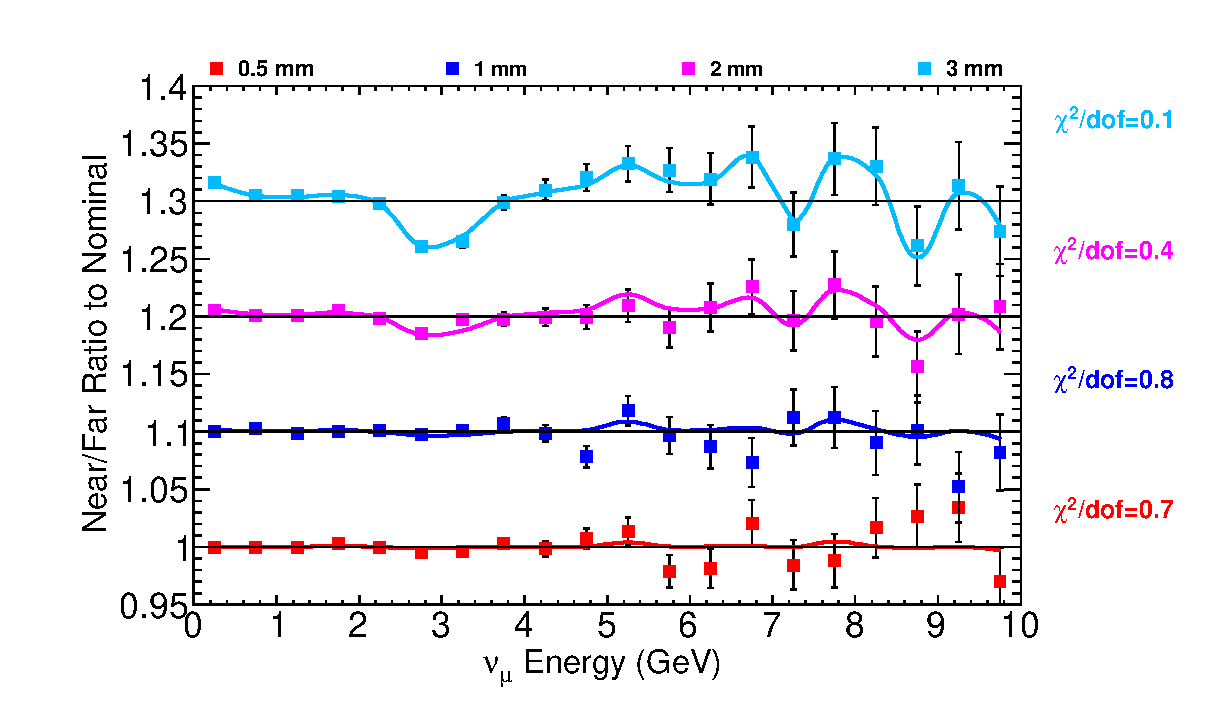
\includegraphics[width=6.0in]{figures/TargetXTilt_nof_summary.eps}}
  \end{center}
\caption{ Near/Far double ratios to nominal for several values of {\bf Target Tilt in $x$} (points) and the results of the fits to each energy bin (lines).}
\end{figure}

\begin{figure}[ht]
  \begin{center}
    {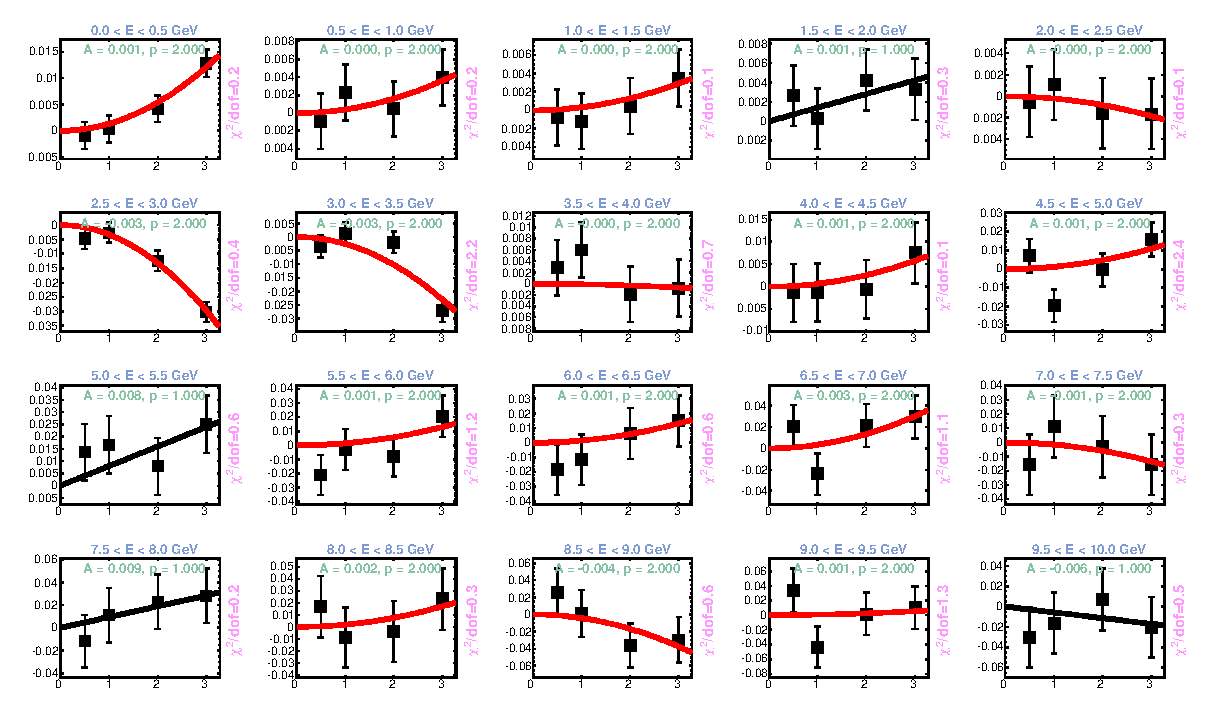
\includegraphics[width=5.0in]{figures/TargetXTilt_nof_fits.eps}}
  \end{center}
\caption{ Fits to the near/far ratios for several values of {\bf Target Tilt in $x$}. Black(Red) fit lines indicate that a linear(parabolic) fit provided the best $\chi^2$. }
\end{figure}

\clearpage

\begin{figure}[ht]
  \begin{center}
    {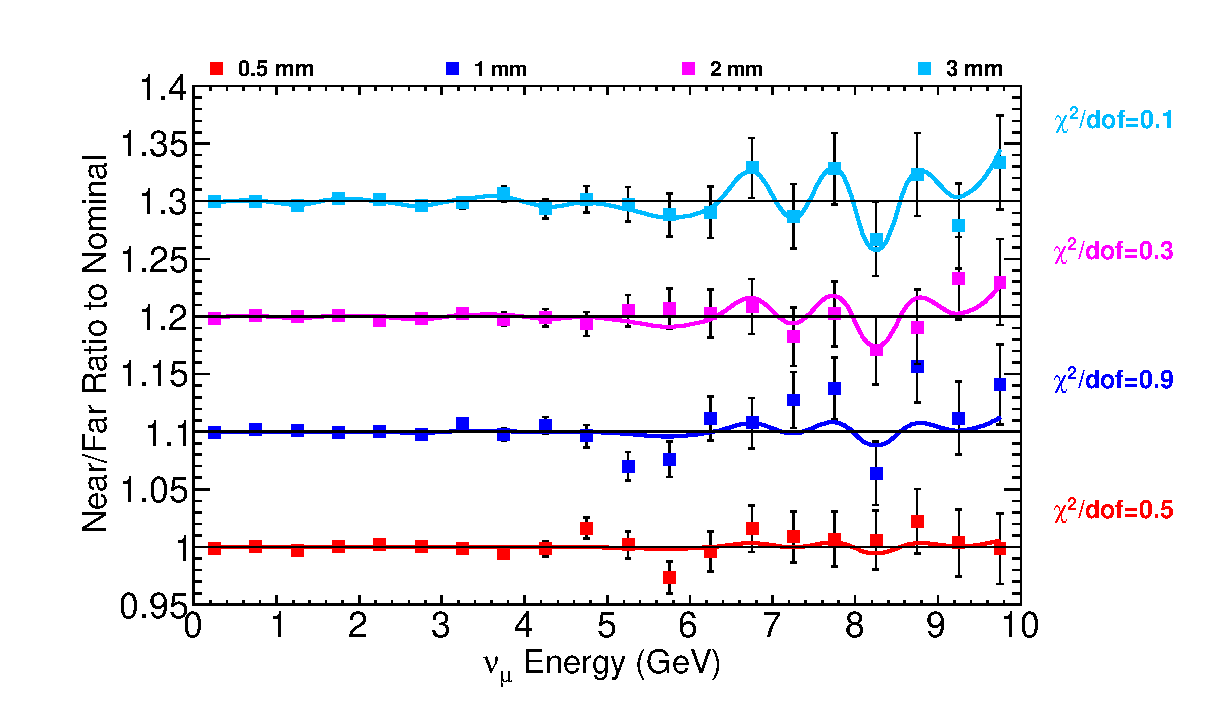
\includegraphics[width=6.0in]{figures/TargetYTilt_nof_summary.eps}}
  \end{center}
\caption{ Near/Far double ratios to nominal for several values of {\bf Target Tilt in $y$} (points) and the results of the fits to each energy bin (lines).}
\end{figure}

\begin{figure}[ht]
  \begin{center}
    {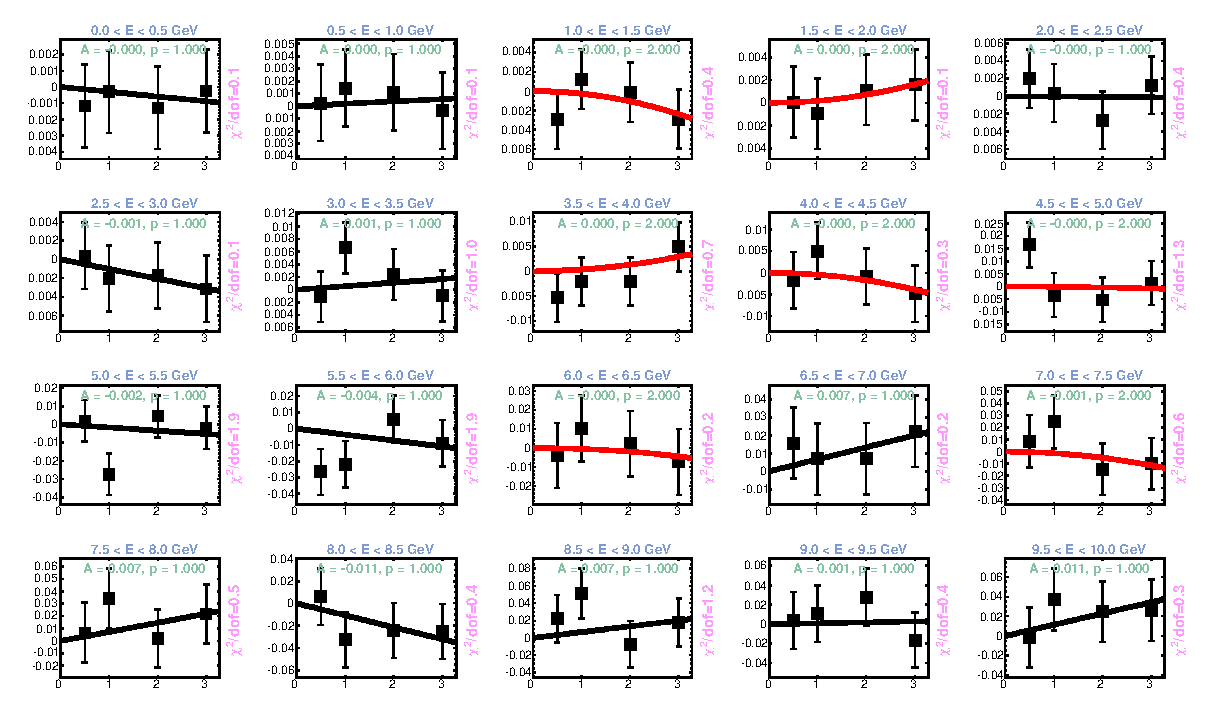
\includegraphics[width=5.0in]{figures/TargetYTilt_nof_fits.eps}}
  \end{center}
\caption{ Fits to the near/far ratios for several values of {\bf Target Tilt in $y$}. Black(Red) fit lines indicate that a linear(parabolic) fit provided the best $\chi^2$. }
\end{figure}


\begin{figure}[ht]
  \begin{center}
    {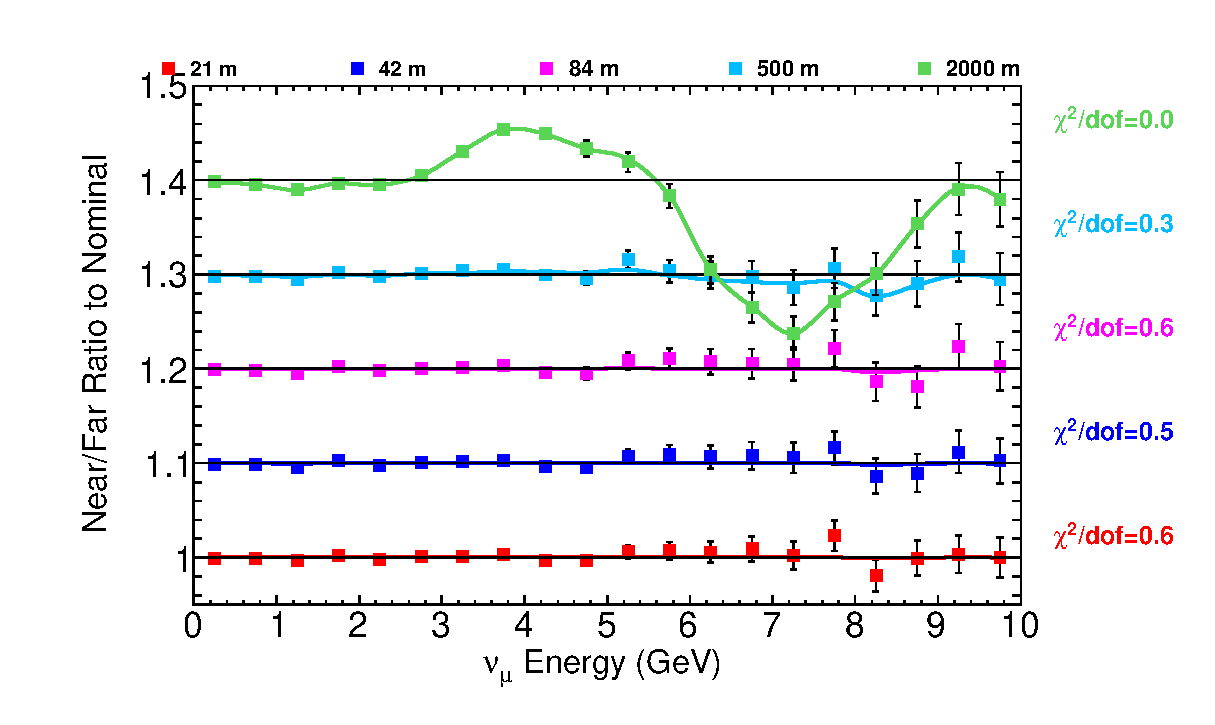
\includegraphics[width=6.0in]{figures/LBNEFDX_nof_summary.eps}}
  \end{center}
\caption{ Near/Far double ratios to nominal for several values of {\bf Far detector offset in $x$} (points) and the results of the fits to each energy bin (lines).}
\end{figure}

\begin{figure}[ht]
  \begin{center}
    {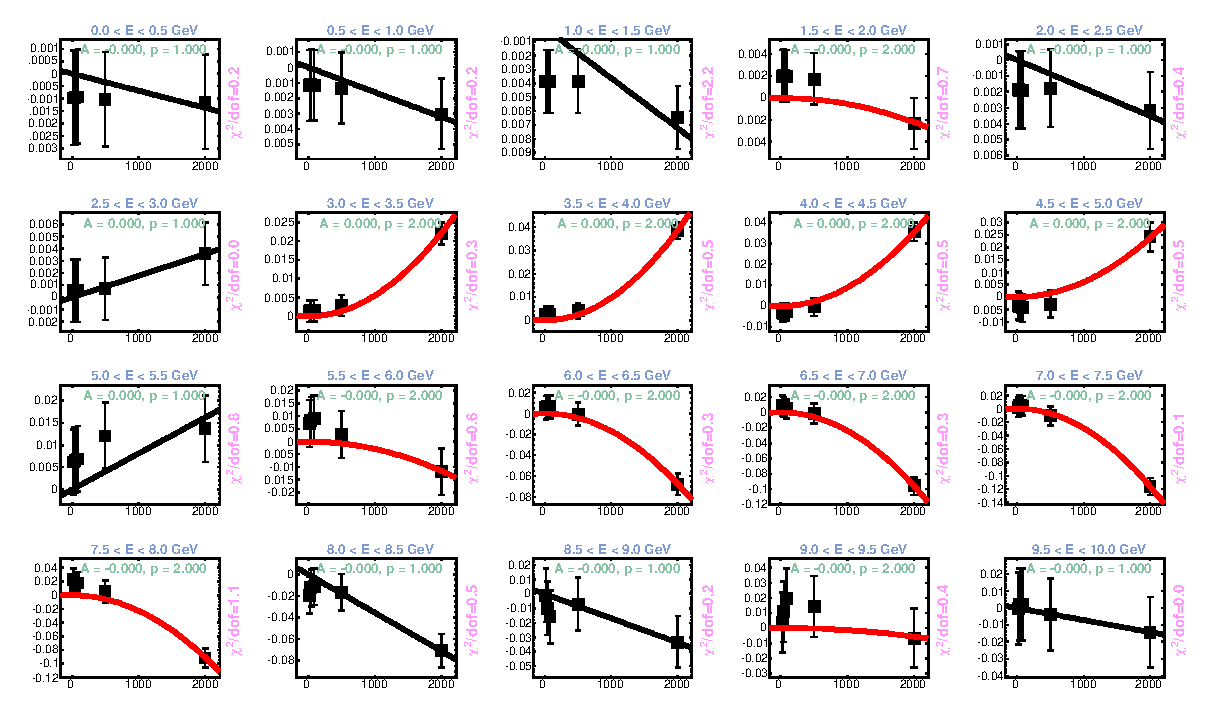
\includegraphics[width=5.0in]{figures/LBNEFDX_nof_fits.eps}}
  \end{center}
\caption{ Fits to the near/far ratios for several values of {\bf Far detector offset in $x$}. Black(Red) fit lines indicate that a linear(parabolic) fit provided the best $\chi^2$. }
\end{figure}

\begin{figure}[ht]
  \begin{center}
    {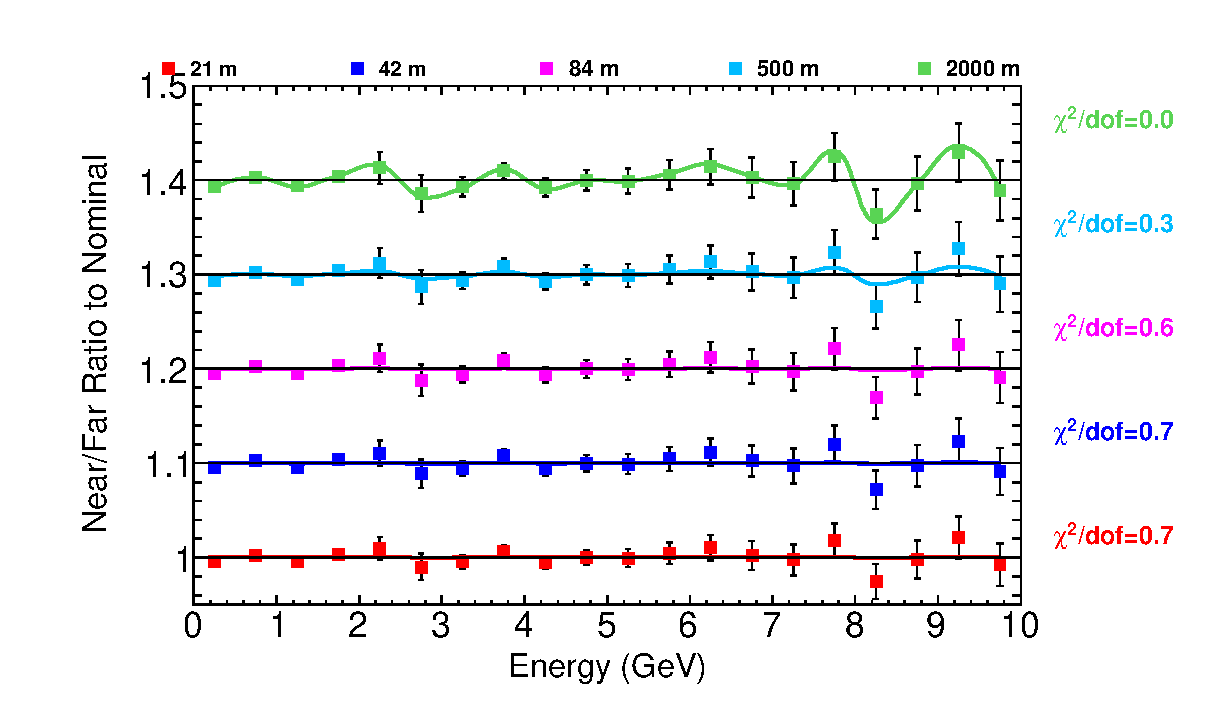
\includegraphics[width=6.0in]{figures/LBNEFDY_nof_summary.eps}}
  \end{center}
\caption{ Near/Far double ratios to nominal for several values of {\bf Far detector offset in $y$} (points) and the results of the fits to each energy bin (lines).}
\end{figure}

\begin{figure}[ht]
  \begin{center}
    {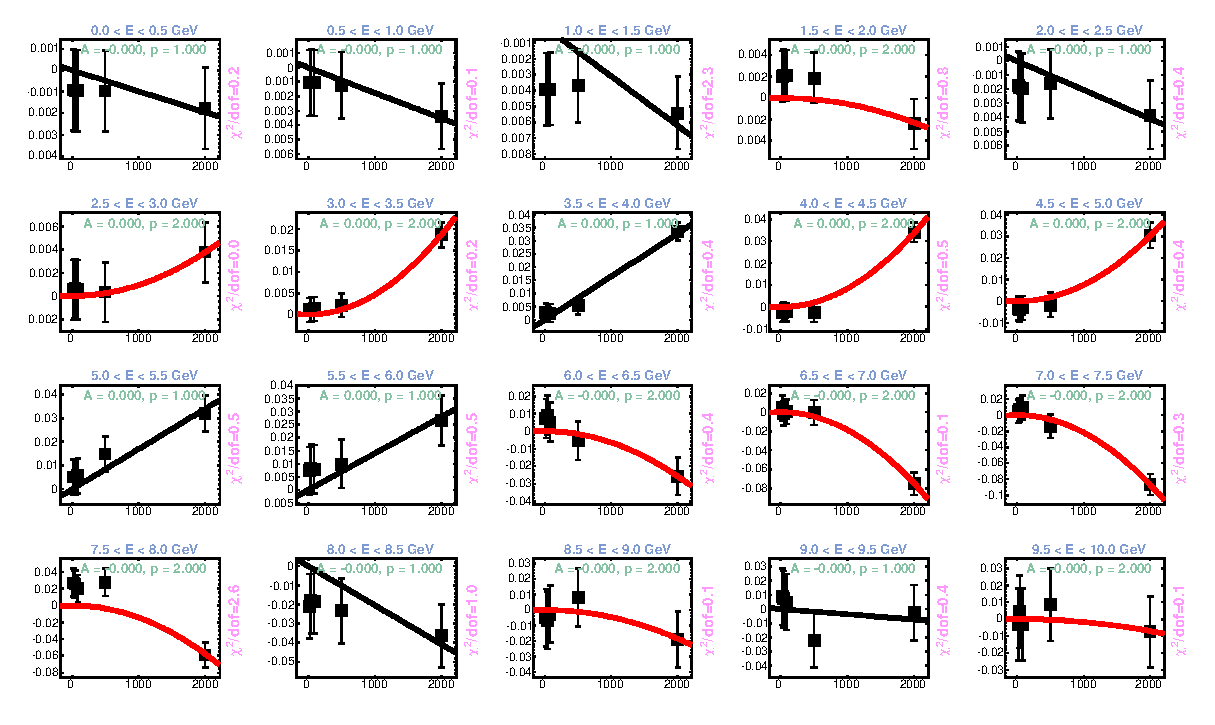
\includegraphics[width=5.0in]{figures/LBNEFDY_nof_fits.eps}}
  \end{center}
\caption{ Fits to the near/far ratios for several values of {\bf Far detector offset in $y$}. Black(Red) fit lines indicate that a linear(parabolic) fit provided the best $\chi^2$. }
\end{figure}

\begin{figure}[ht]
  \begin{center}
    {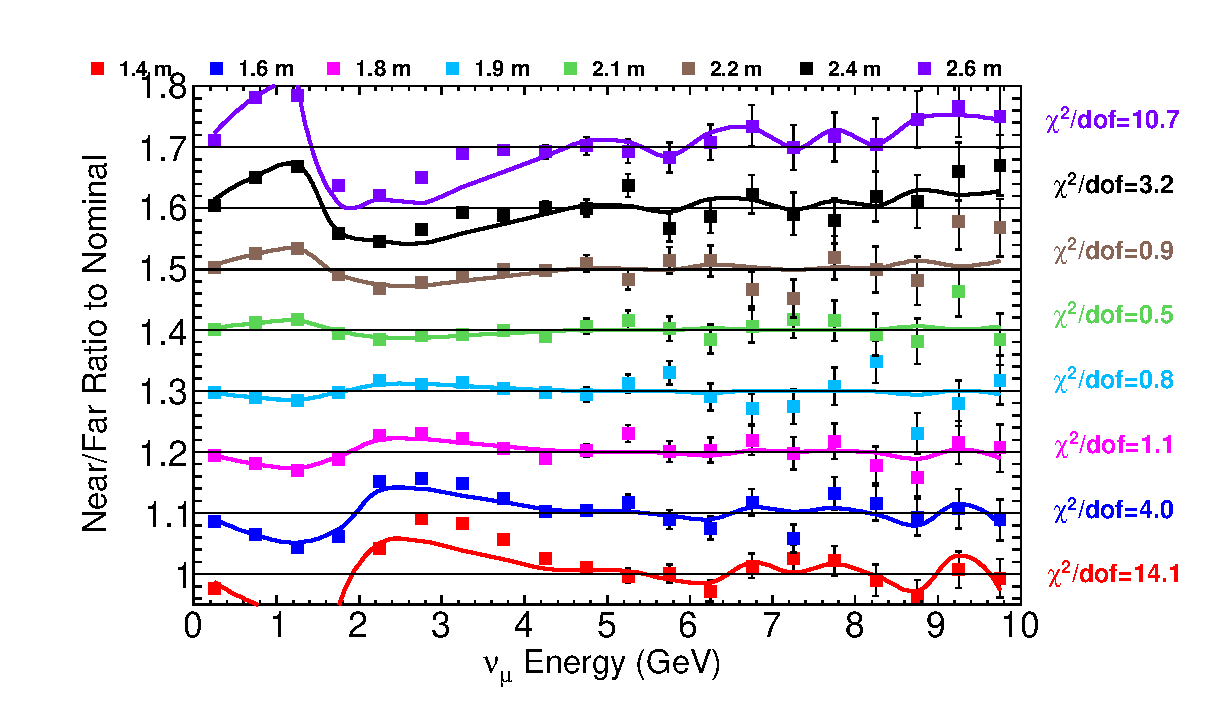
\includegraphics[width=6.0in]{figures/DecayPipeRadius_nof_summary.eps}}
  \end{center}
\caption{ Near/Far double ratios to nominal for several values of {\bf Decay Pipe Radius} (points) and the results of the fits to each energy bin (lines).}
\end{figure}

\begin{figure}[ht]
  \begin{center}
    {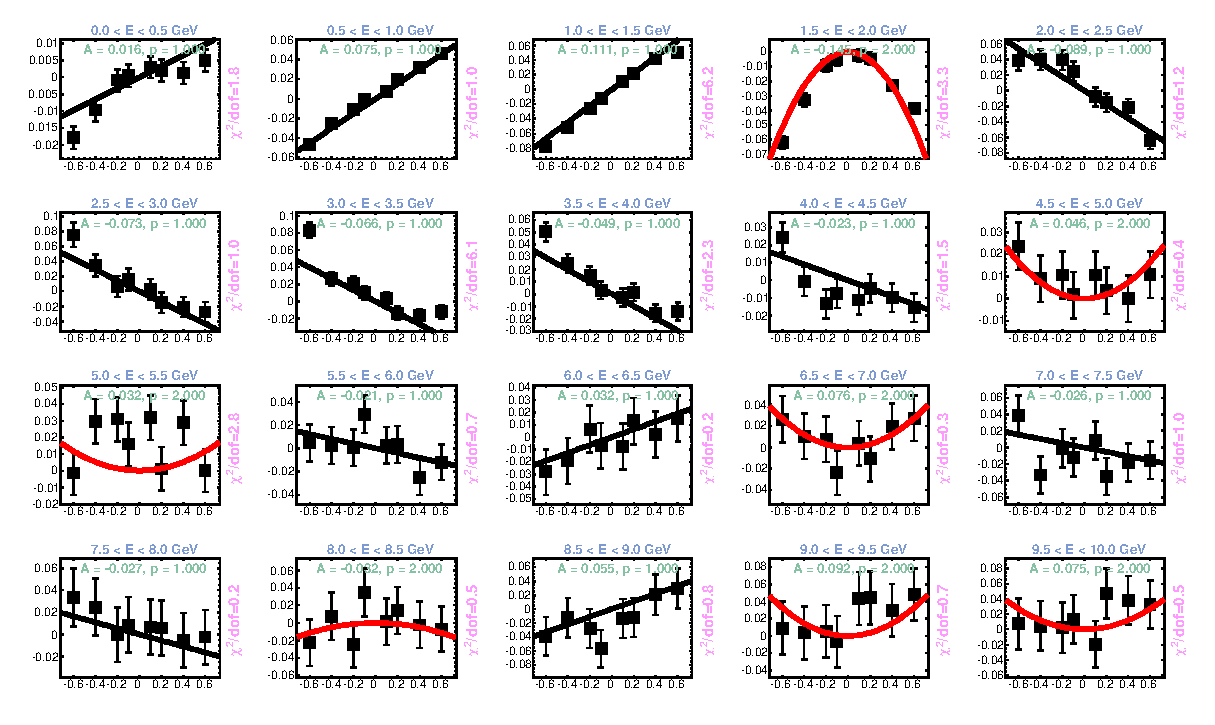
\includegraphics[width=5.0in]{figures/DecayPipeRadius_nof_fits.eps}}
  \end{center}
\caption{ Fits to the near/far ratios for several values of {\bf Decay Pipe Radius}. Black(Red) fit lines indicate that a linear(parabolic) fit provided the best $\chi^2$. }
\end{figure}

\begin{figure}[ht]
  \begin{center}
    {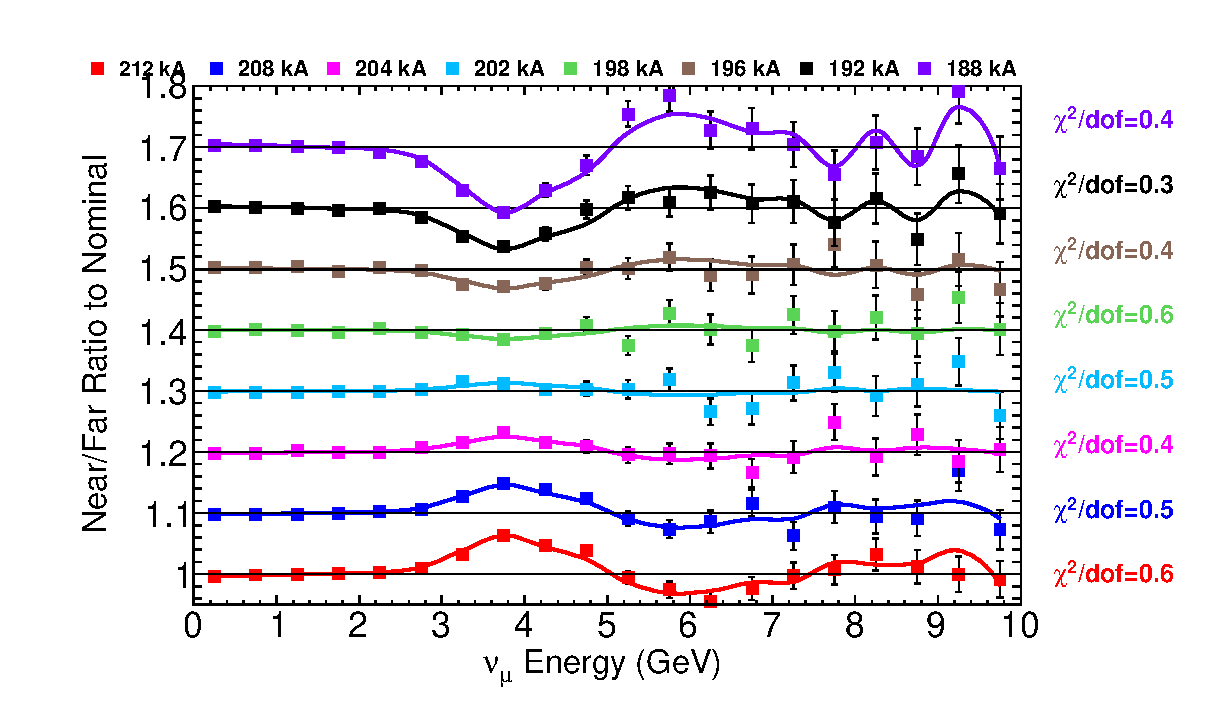
\includegraphics[width=6.0in]{figures/HornCurrent_nof_summary.eps}}
  \end{center}
\caption{ Near/Far double ratios to nominal for several values of {\bf Horn Current} (points) and the results of the fits to each energy bin (lines).}
\end{figure}

\begin{figure}[ht]
  \begin{center}
    {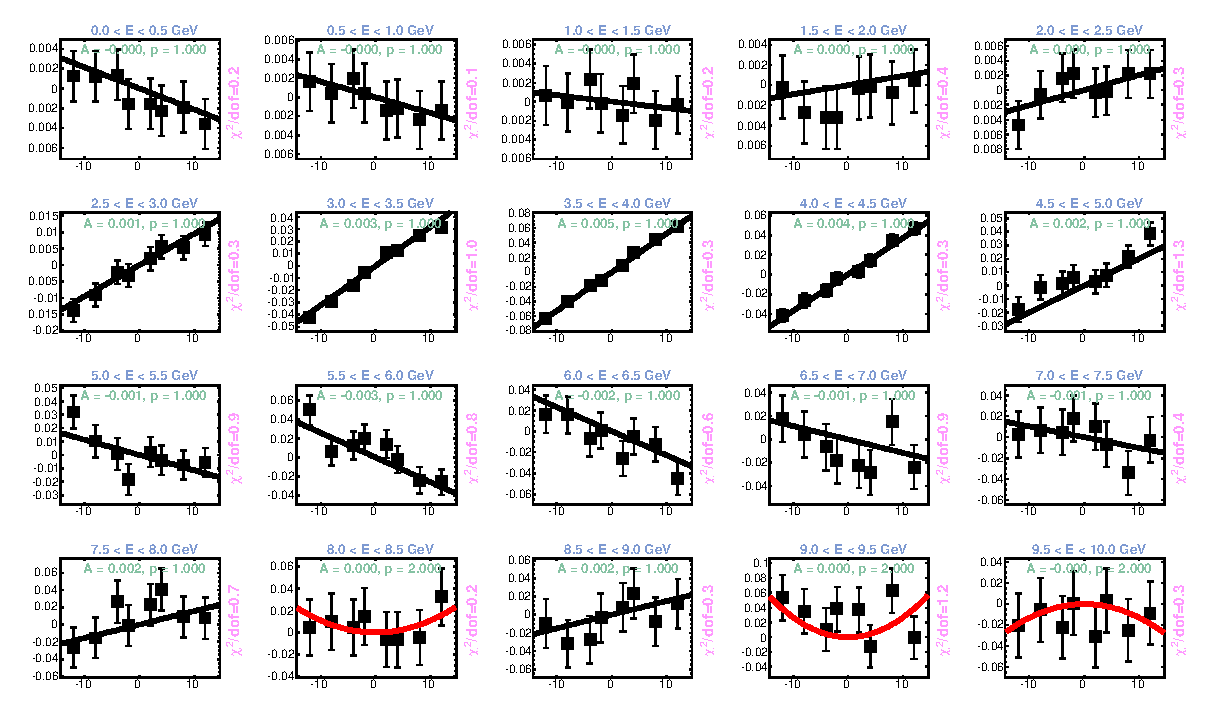
\includegraphics[width=5.0in]{figures/HornCurrent_nof_fits.eps}}
  \end{center}
\caption{ Fits to the near/far ratios for several values of {\bf HornCurrent}. Black(Red) fit lines indicate that a linear(parabolic) fit provided the best $\chi^2$. }
\end{figure}

\begin{figure}[ht]
  \begin{center}
    {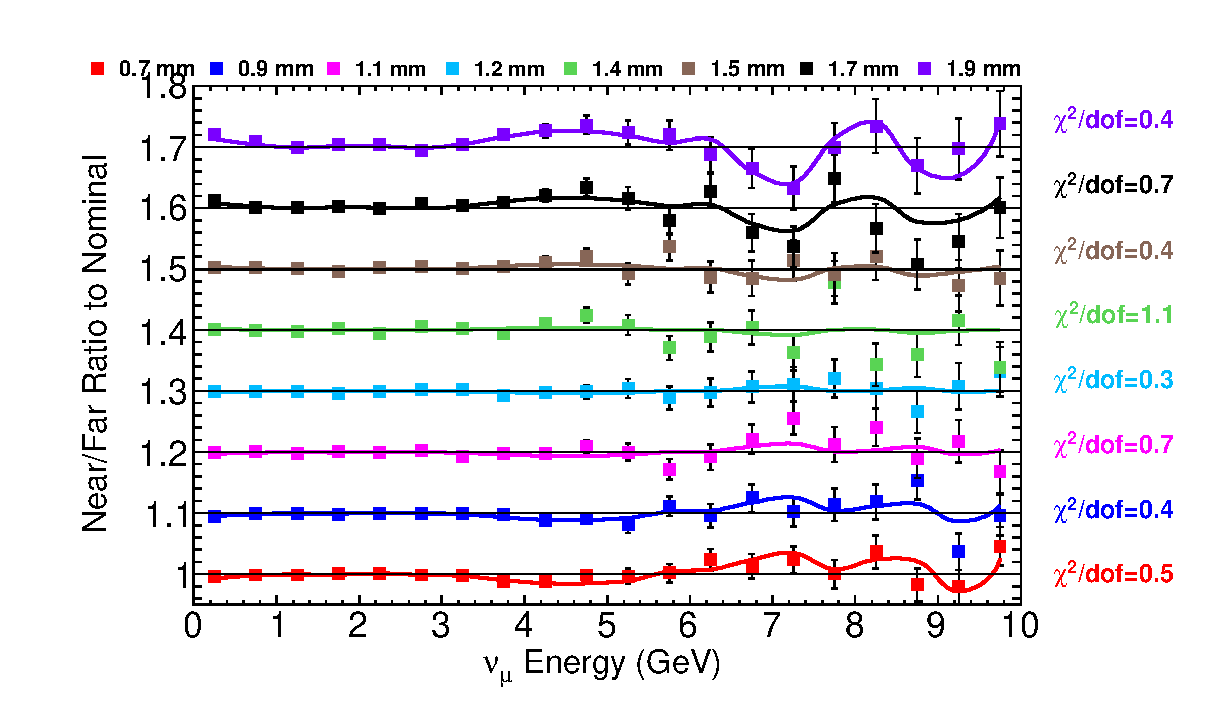
\includegraphics[width=6.0in]{figures/BeamSigmaX_nof_summary.eps}}
  \end{center}
\caption{ Near/Far double ratios to nominal for several values of {\bf Beam size in $x$} (points) and the results of the fits to each energy bin (lines).}
\end{figure}

\begin{figure}[ht]
  \begin{center}
    {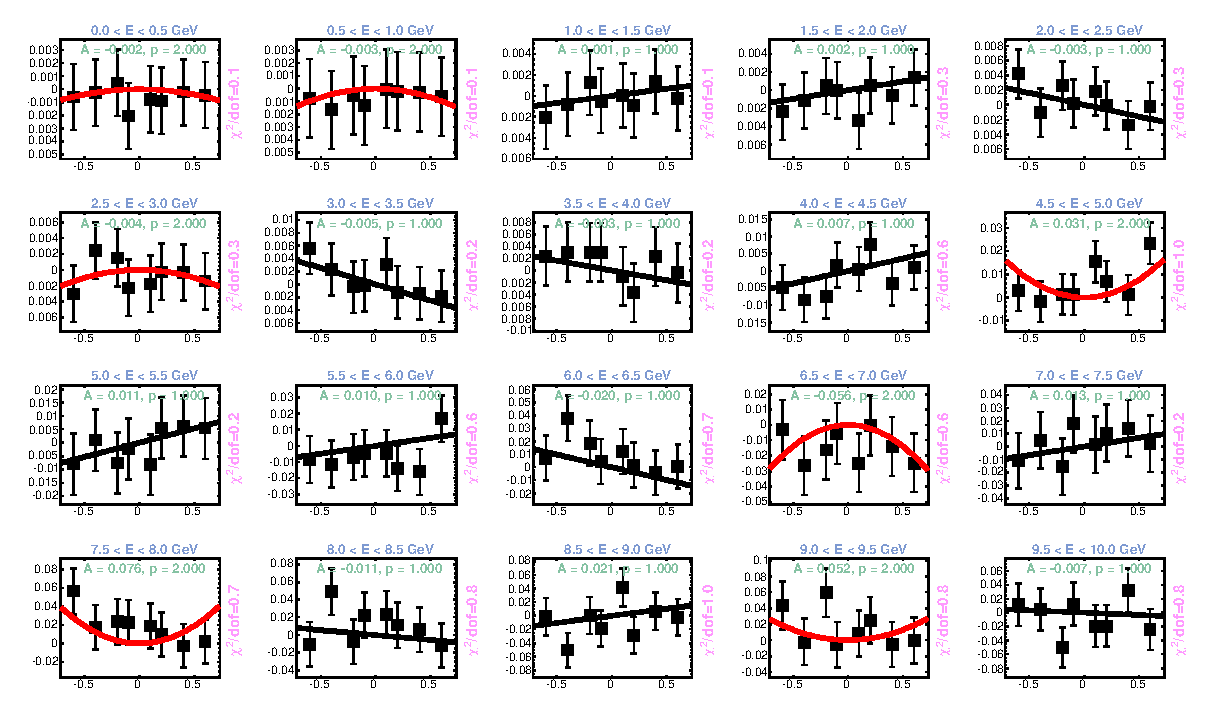
\includegraphics[width=5.0in]{figures/BeamSigmaY_nof_fits.eps}}
  \end{center}
\caption{ Fits to the near/far ratios for several values of {\bf Beam size in $y$}. Black(Red) fit lines indicate that a linear(parabolic) fit provided the best $\chi^2$. }
\end{figure}

\clearpage

\begin{figure}[ht]
  \begin{center}
    {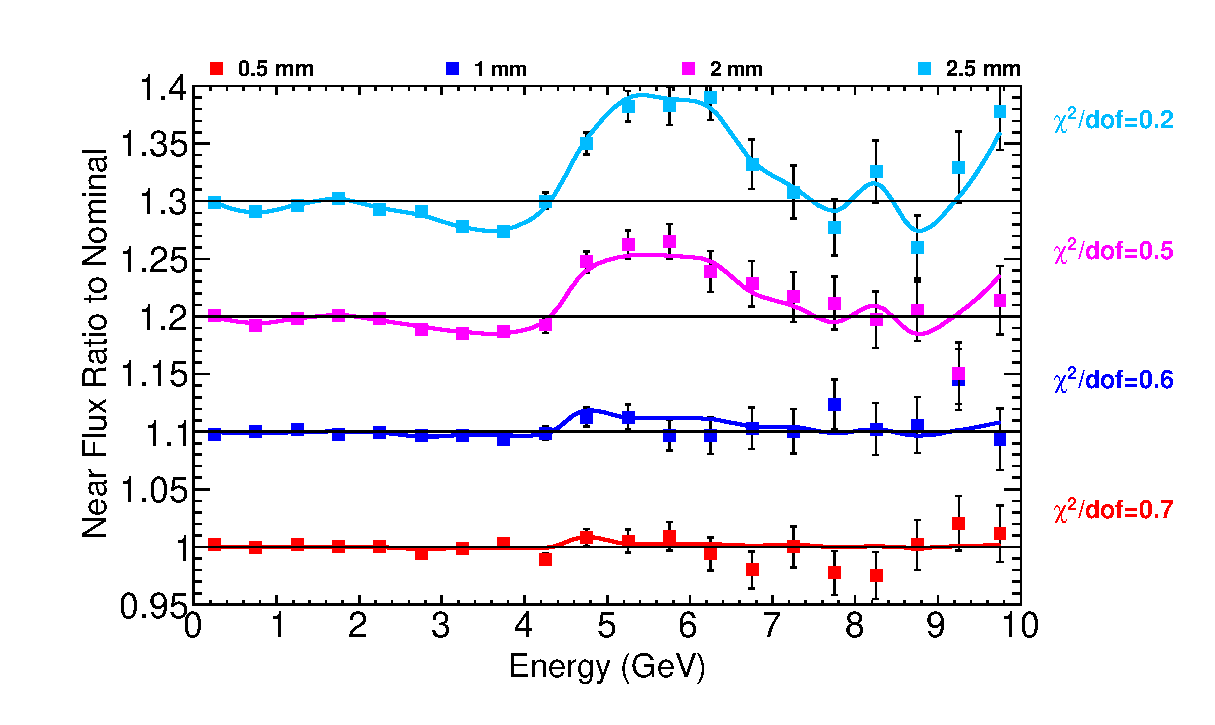
\includegraphics[width=6.0in]{figures/Horn1XOffset_near_summary.eps}}
  \end{center}
\caption{ Near detector flux ratios to nominal for several values of {\bf Horn 1 Offset in $x$} (points) and the results of the fits to each energy bin (lines).}
\end{figure}

\begin{figure}[ht]
  \begin{center}
    {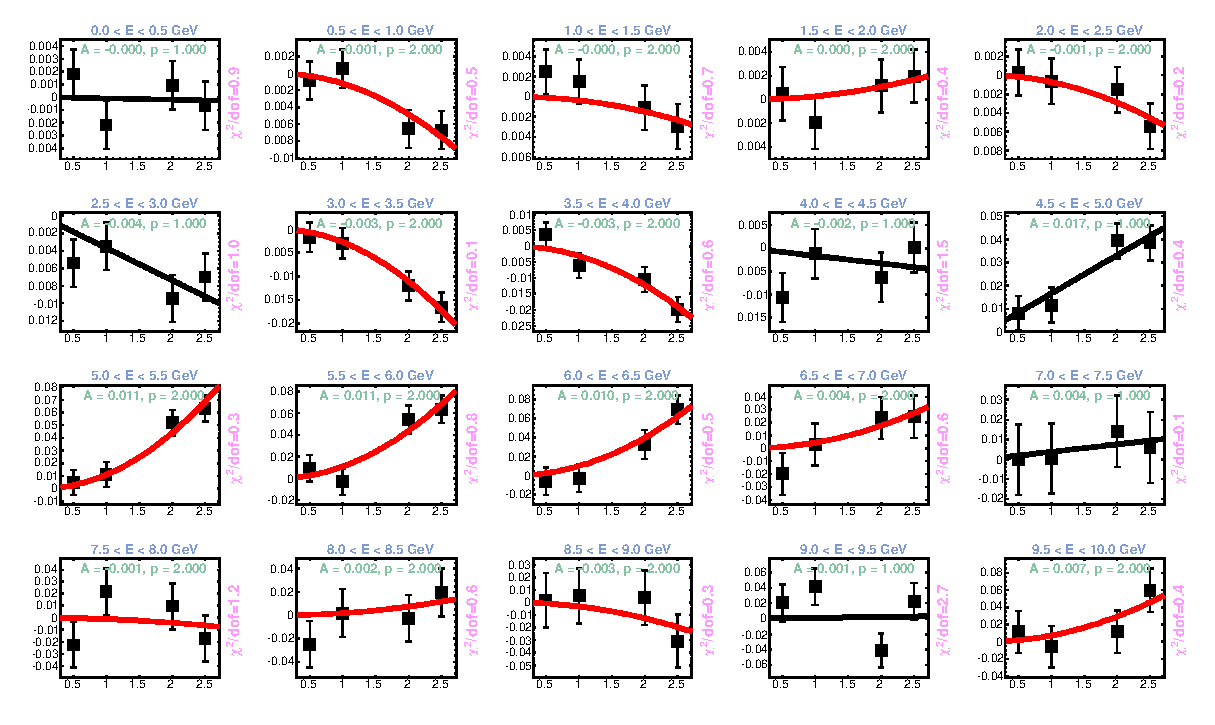
\includegraphics[width=5.0in]{figures/Horn1XOffset_near_fits.eps}}
  \end{center}
\caption{ Fits to the far flux ratios for several values of {\bf Horn 1 Offset in $x$}. Black(Red) fit lines indicate that a linear(parabolic) fit provided the best $\chi^2$. }
\end{figure}

\begin{figure}[ht]
  \begin{center}
    {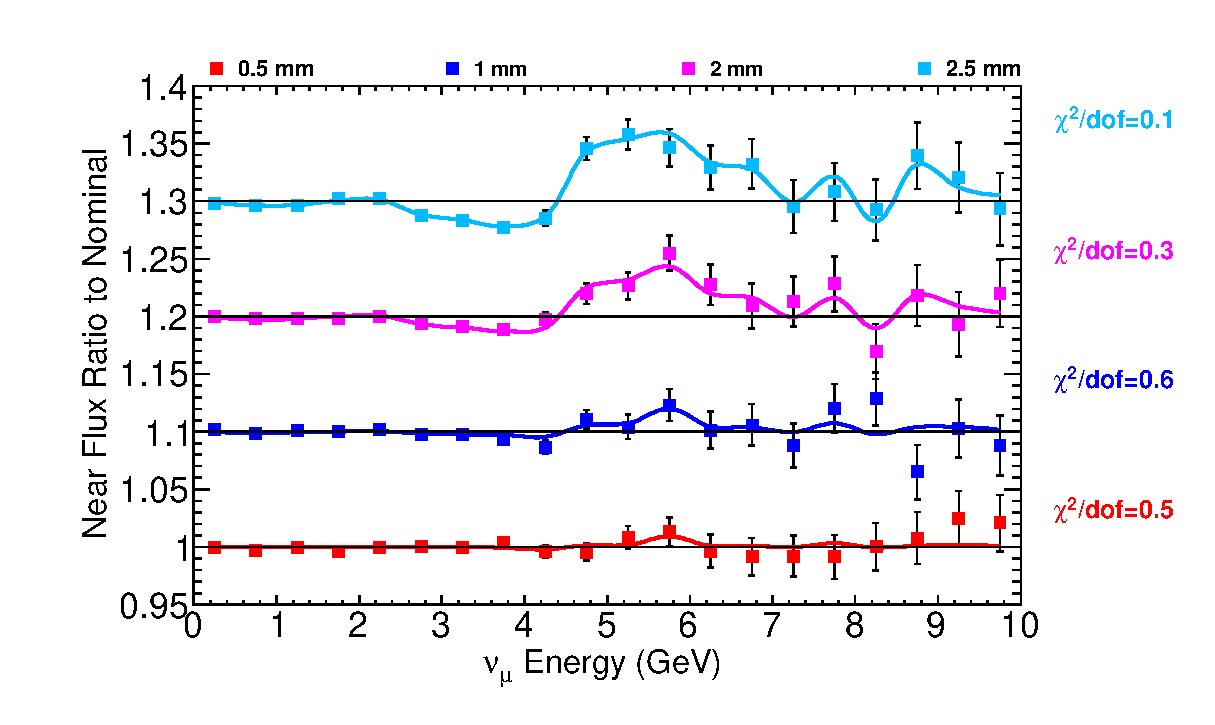
\includegraphics[width=6.0in]{figures/Horn1YOffset_near_summary.eps}}
  \end{center}
\caption{ Near detector flux ratios to nominal for several values of {\bf Horn 1 Offset in $y$} (points) and the results of the fits to each energy bin (lines).}
\end{figure}

\begin{figure}[ht]
  \begin{center}
    {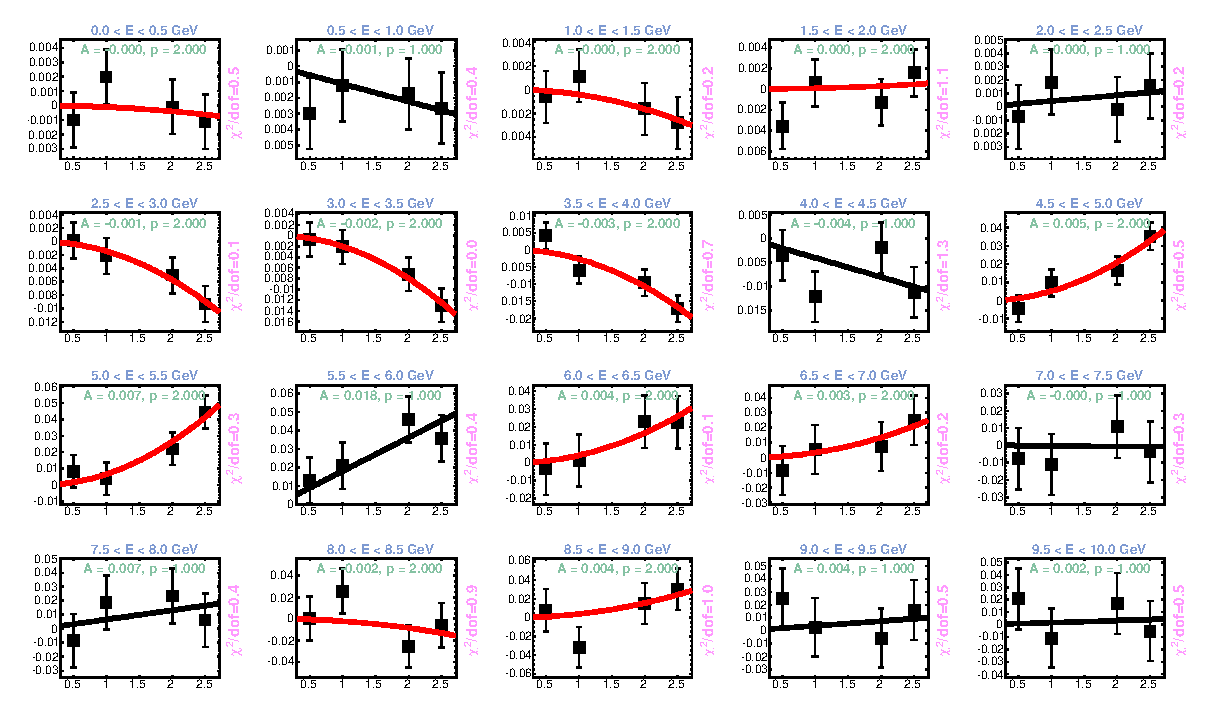
\includegraphics[width=5.0in]{figures/Horn1YOffset_near_fits.eps}}
  \end{center}
\caption{ Fits to the near flux ratios for several values of {\bf Horn 1 Offset in $y$}. Black(Red) fit lines indicate that a linear(parabolic) fit provided the best $\chi^2$. }
\end{figure}

\begin{figure}[ht]
  \begin{center}
    {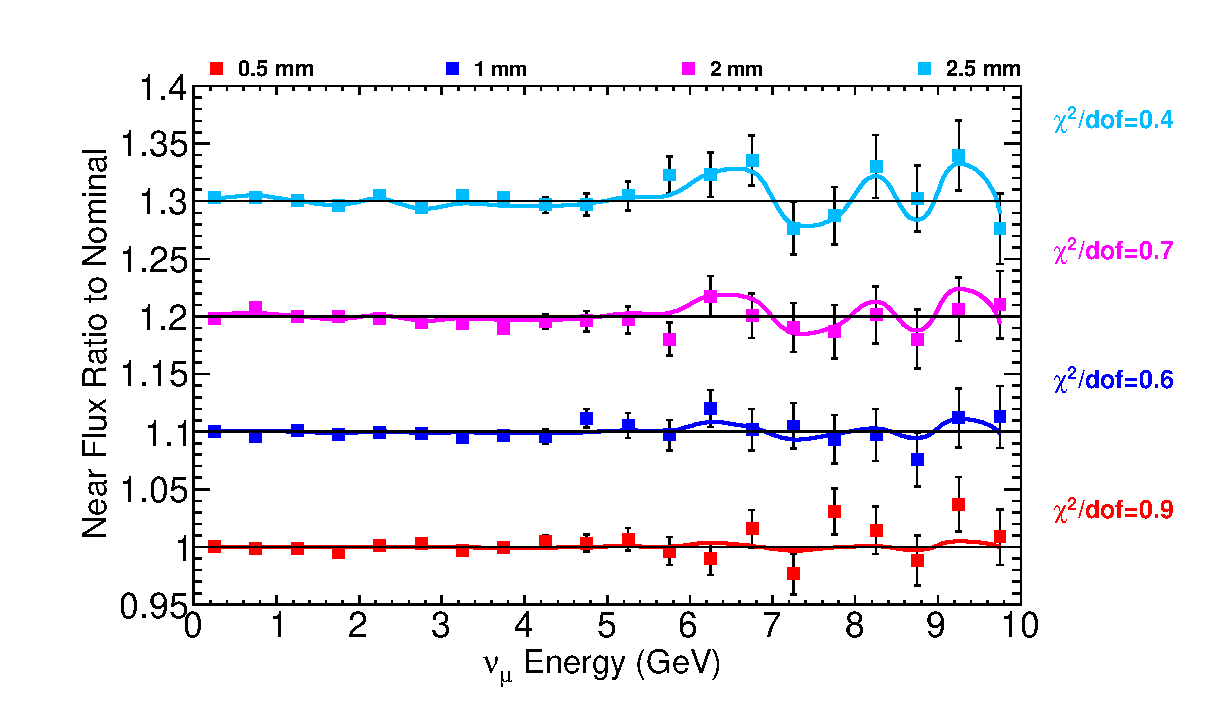
\includegraphics[width=6.0in]{figures/Horn2XOffset_near_summary.eps}}
  \end{center}
\caption{ Near detector flux ratios to nominal for several values of {\bf Horn 2 Offset in $x$} (points) and the results of the fits to each energy bin (lines).}
\end{figure}

\begin{figure}[ht]
  \begin{center}
    {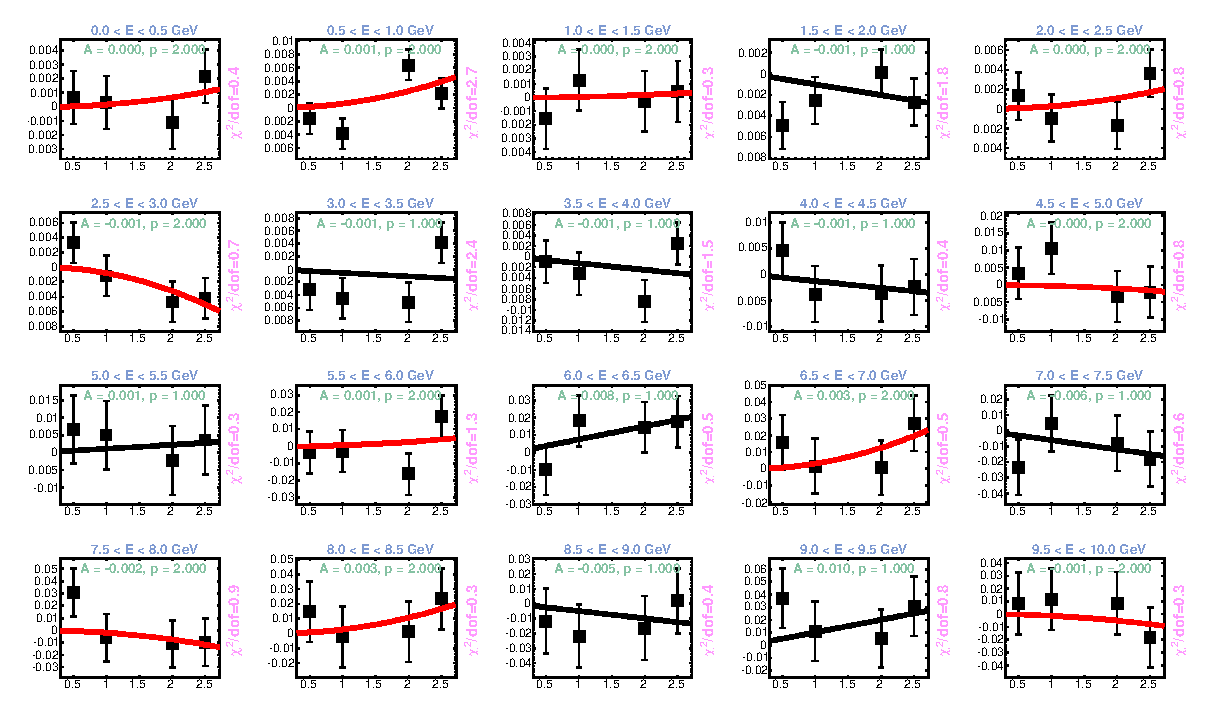
\includegraphics[width=5.0in]{figures/Horn2XOffset_near_fits.eps}}
  \end{center}
\caption{ Fits to the near flux ratios for several values of {\bf Horn 2 Offset in $x$}. Black(Red) fit lines indicate that a linear(parabolic) fit provided the best $\chi^2$. }
\end{figure}

\begin{figure}[ht]
  \begin{center}
    {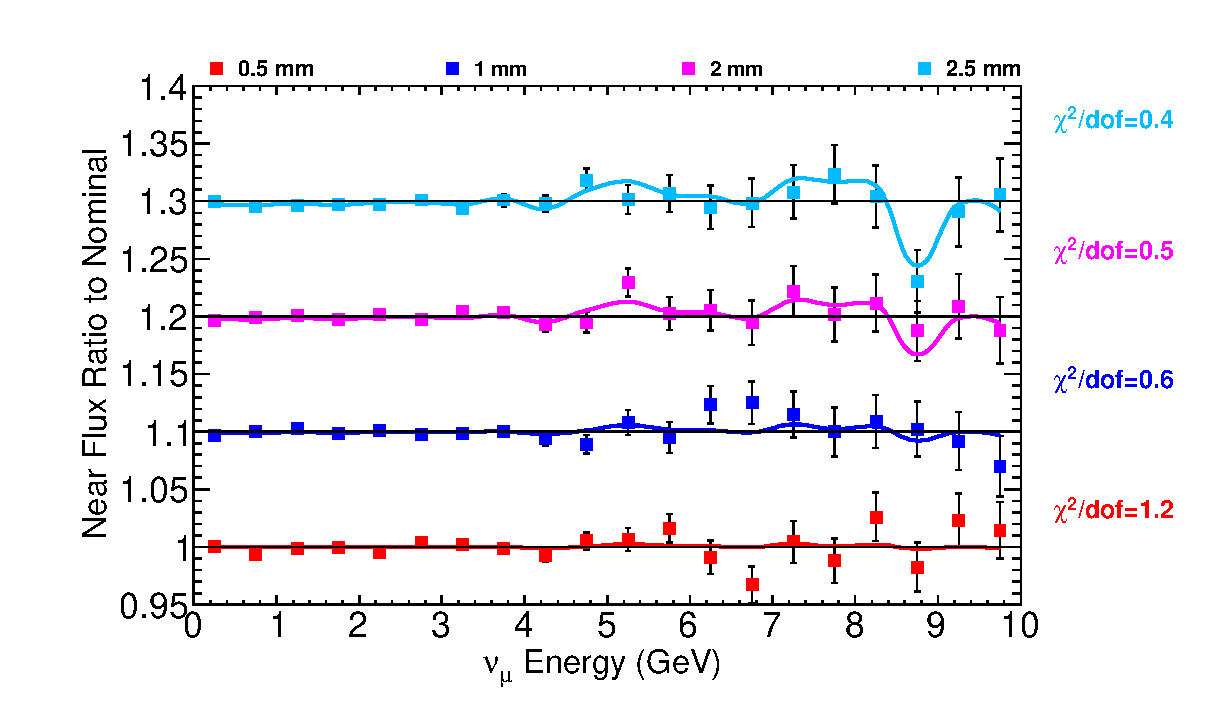
\includegraphics[width=6.0in]{figures/Horn2YOffset_near_summary.eps}}
  \end{center}
\caption{ Near detector flux ratios to nominal for several values of {\bf Horn 2 Offset in $y$} (points) and the results of the fits to each energy bin (lines).}
\end{figure}

\begin{figure}[ht]
  \begin{center}
    {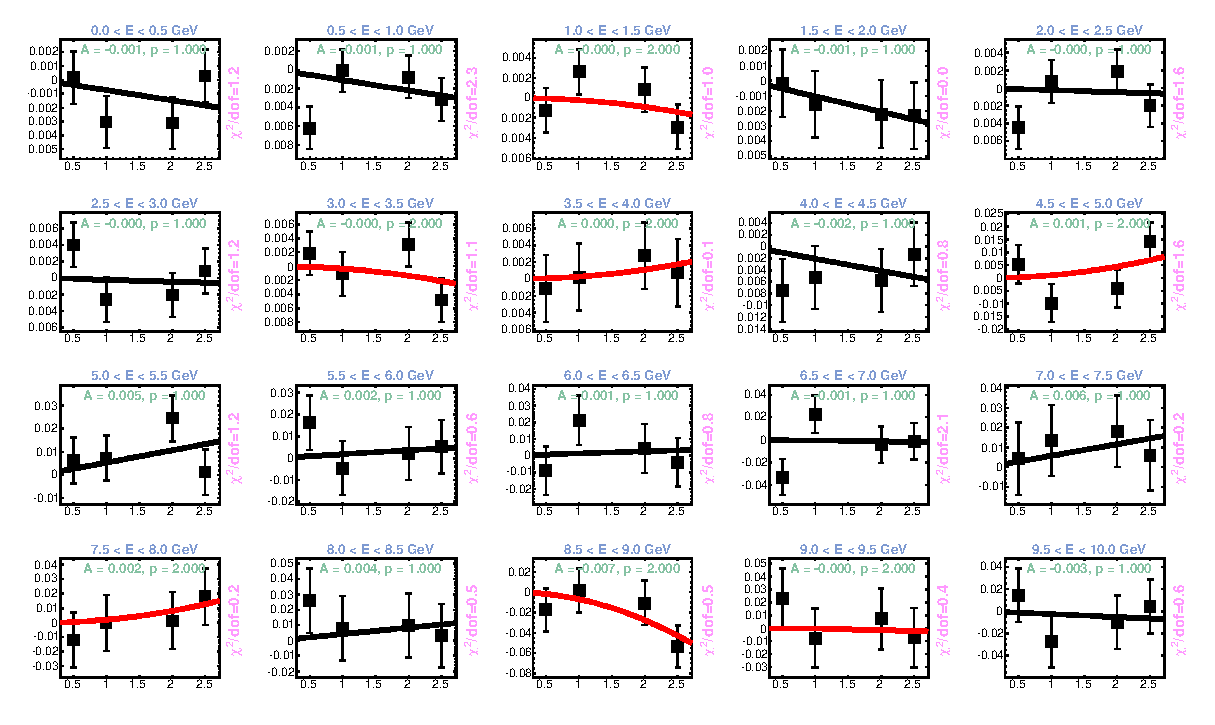
\includegraphics[width=5.0in]{figures/Horn2YOffset_near_fits.eps}}
  \end{center}
\caption{ Fits to the near flux ratios for several values of {\bf Horn 2 Offset in $y$}. Black(Red) fit lines indicate that a linear(parabolic) fit provided the best $\chi^2$. }
\end{figure}

\begin{figure}[ht]
  \begin{center}
    {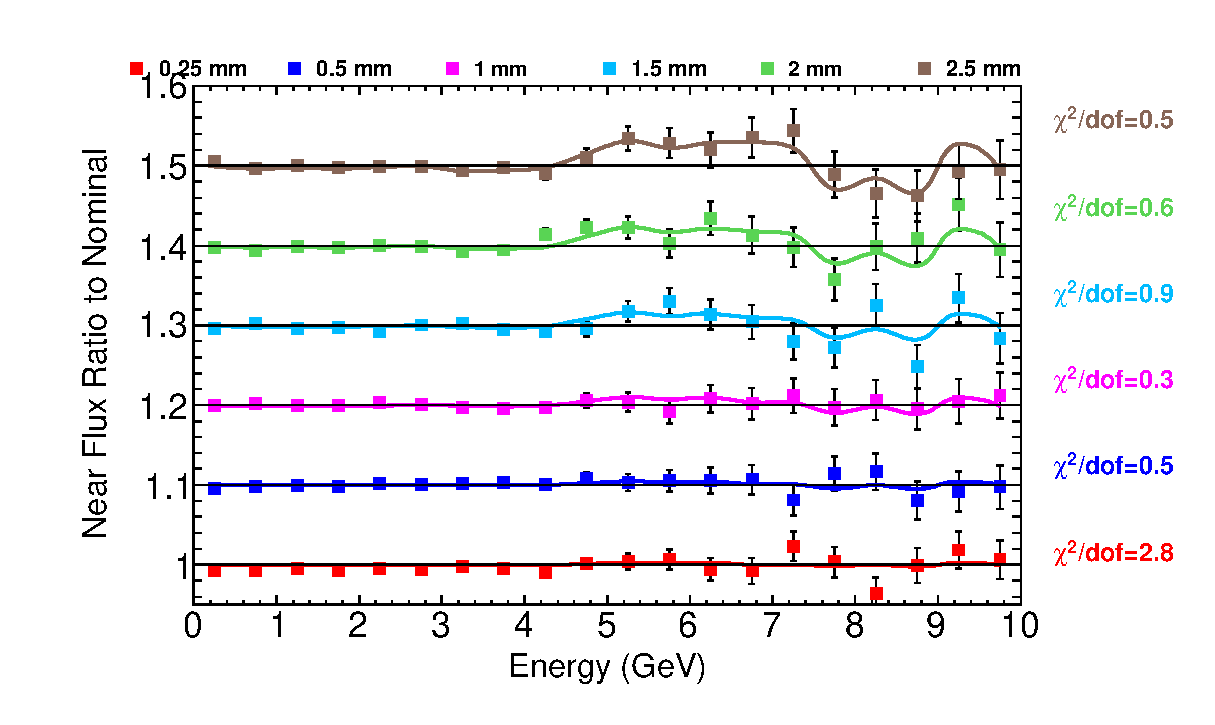
\includegraphics[width=6.0in]{figures/Horn1XTilt_near_summary.eps}}
  \end{center}
\caption{ Near detector flux ratios to nominal for several values of {\bf Horn 1 Tilt in $x$} (points) and the results of the fits to each energy bin (lines).}
\end{figure}

\begin{figure}[ht]
  \begin{center}
    {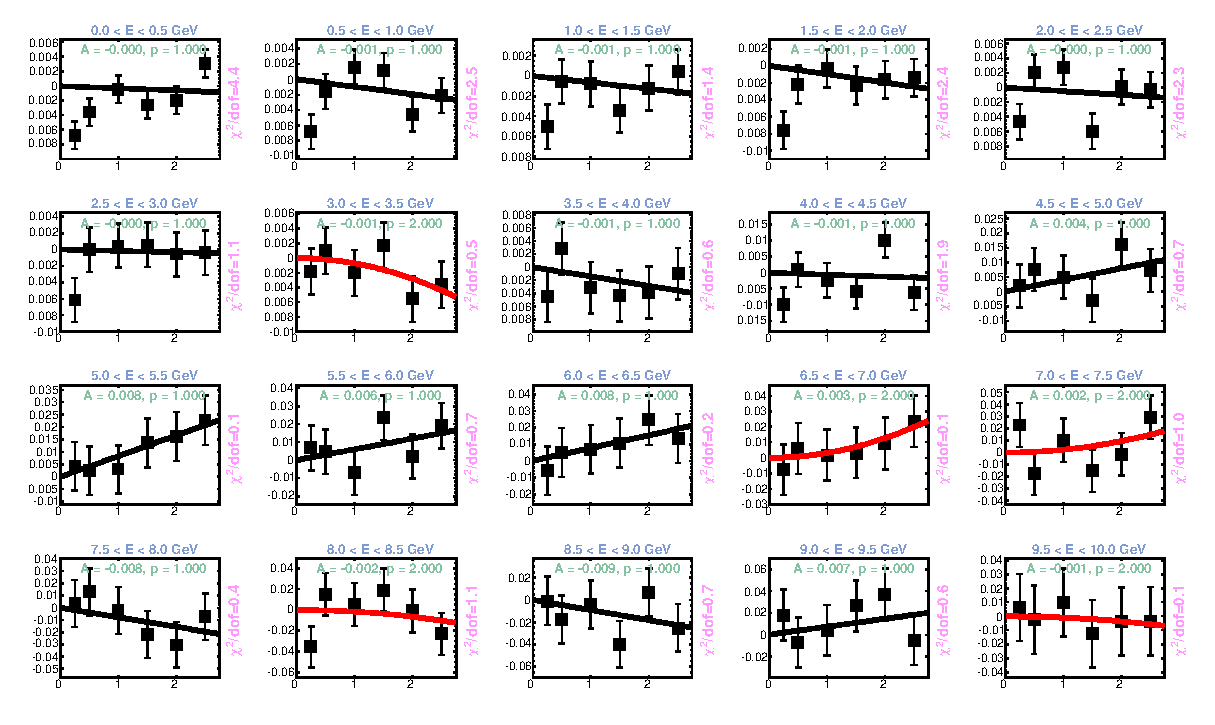
\includegraphics[width=5.0in]{figures/Horn1XTilt_near_fits.eps}}
  \end{center}
\caption{ Fits to the near flux ratios for several values of {\bf Horn 1 Tilt in $x$}. Black(Red) fit lines indicate that a linear(parabolic) fit provided the best $\chi^2$. }
\end{figure}

\begin{figure}[ht]
  \begin{center}
    {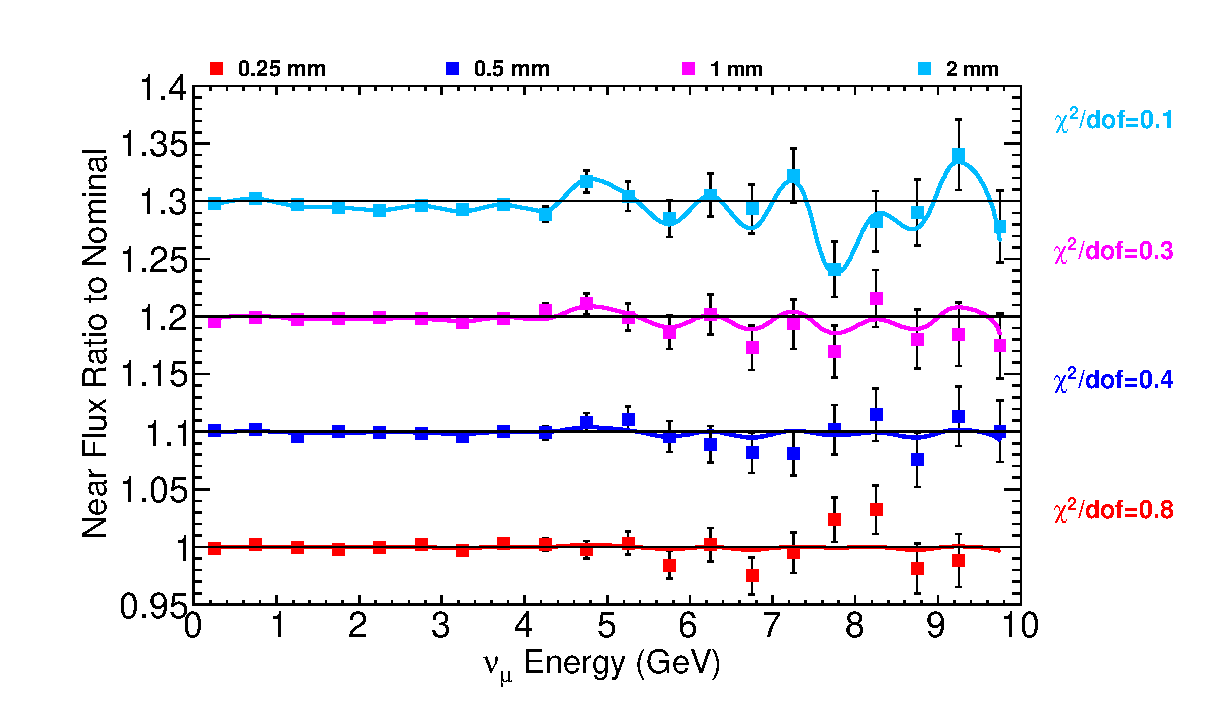
\includegraphics[width=6.0in]{figures/Horn1YTilt_near_summary.eps}}
  \end{center}
\caption{ Near detector flux ratios to nominal for several values of {\bf Horn 1 Tilt in $y$} (points) and the results of the fits to each energy bin (lines).}
\end{figure}

\begin{figure}[ht]
  \begin{center}
    {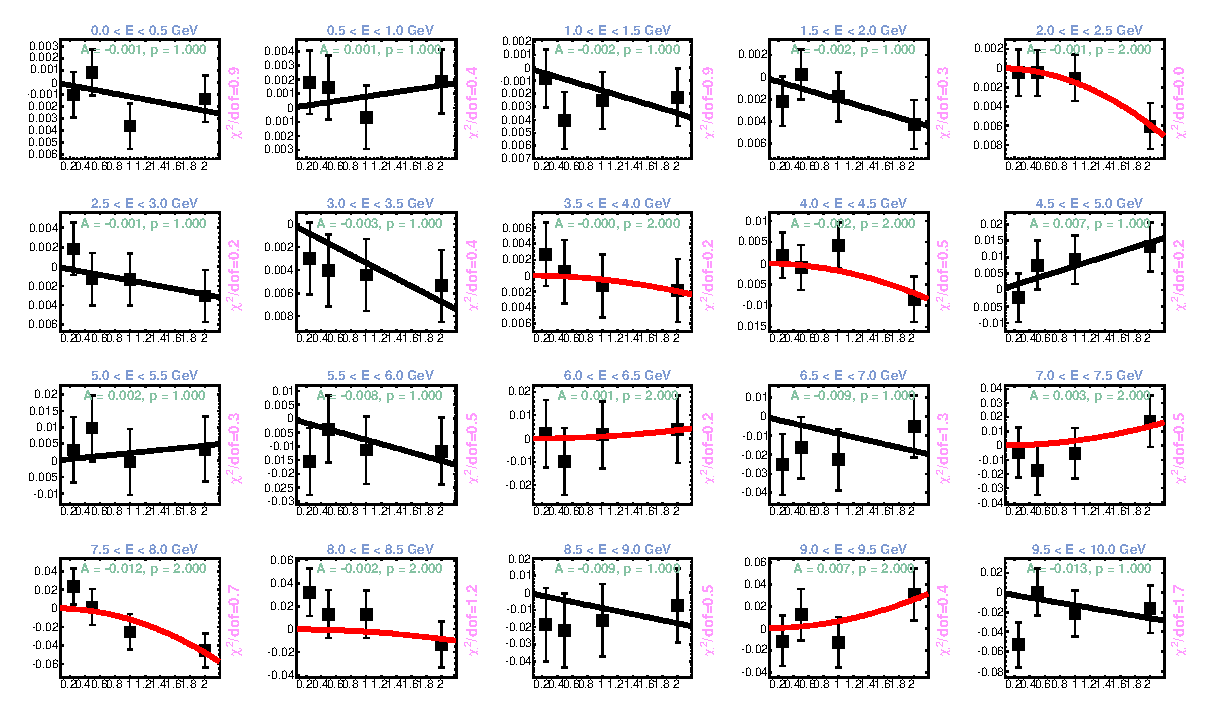
\includegraphics[width=5.0in]{figures/Horn1YTilt_near_fits.eps}}
  \end{center}
\caption{ Fits to the near flux ratios for several values of {\bf Horn 1 Tilt in $y$}. Black(Red) fit lines indicate that a linear(parabolic) fit provided the best $\chi^2$. }
\end{figure}

\clearpage

\begin{figure}[ht]
  \begin{center}
    {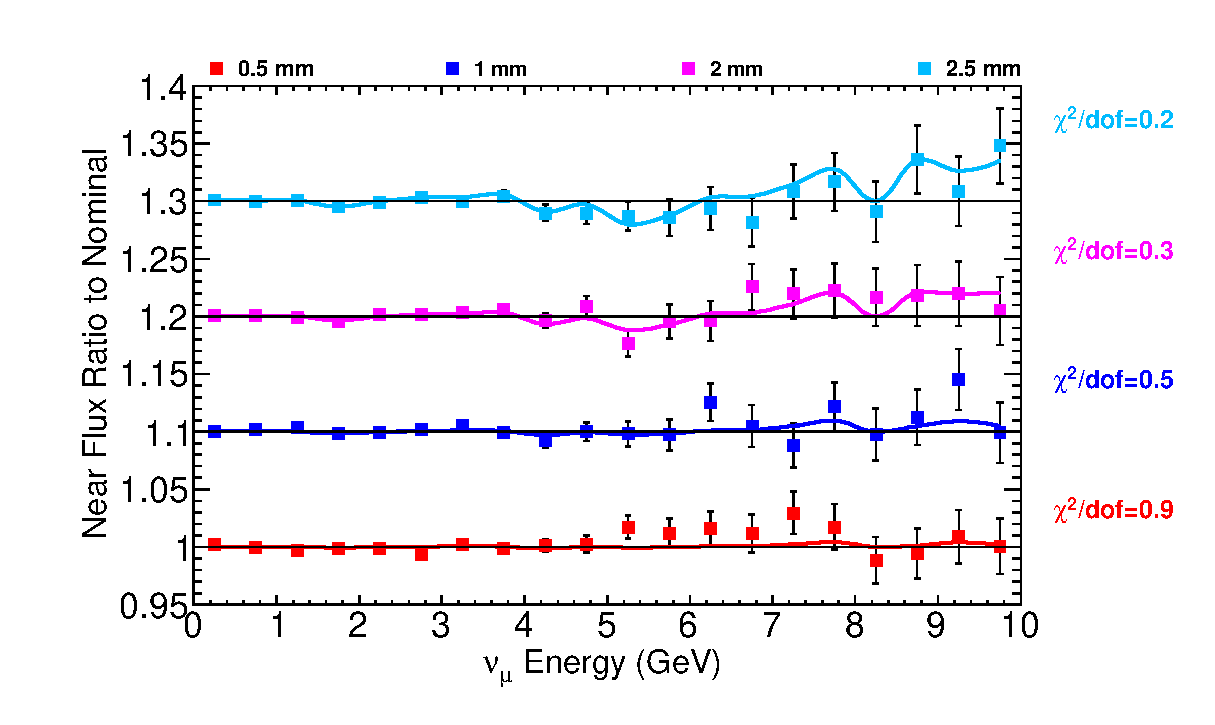
\includegraphics[width=6.0in]{figures/Horn2XTilt_near_summary.eps}}
  \end{center}
\caption{ Near detector flux ratios to nominal for several values of {\bf Horn 2 Tilt in $x$} (points) and the results of the fits to each energy bin (lines).}
\end{figure}

\begin{figure}[ht]
  \begin{center}
    {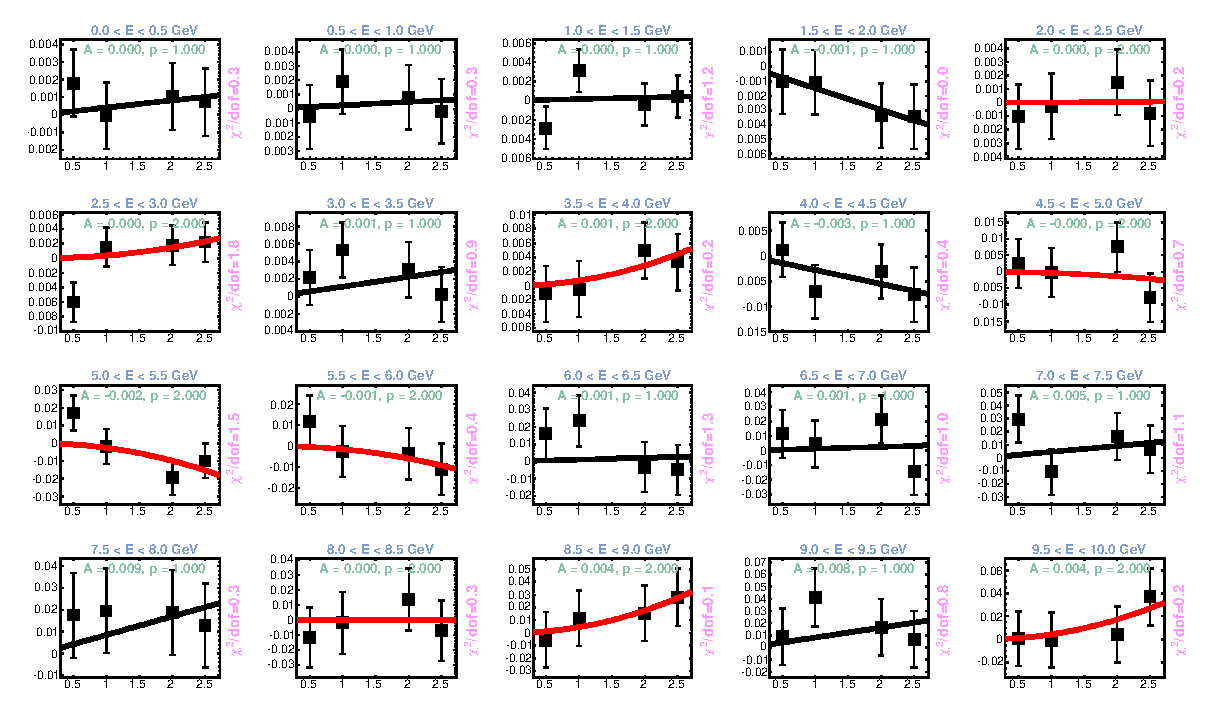
\includegraphics[width=5.0in]{figures/Horn2XTilt_near_fits.eps}}
  \end{center}
\caption{ Fits to the near flux ratios for several values of {\bf Horn 2 Tilt in $x$}. Black(Red) fit lines indicate that a linear(parabolic) fit provided the best $\chi^2$. }
\end{figure}

\begin{figure}[ht]
  \begin{center}
    {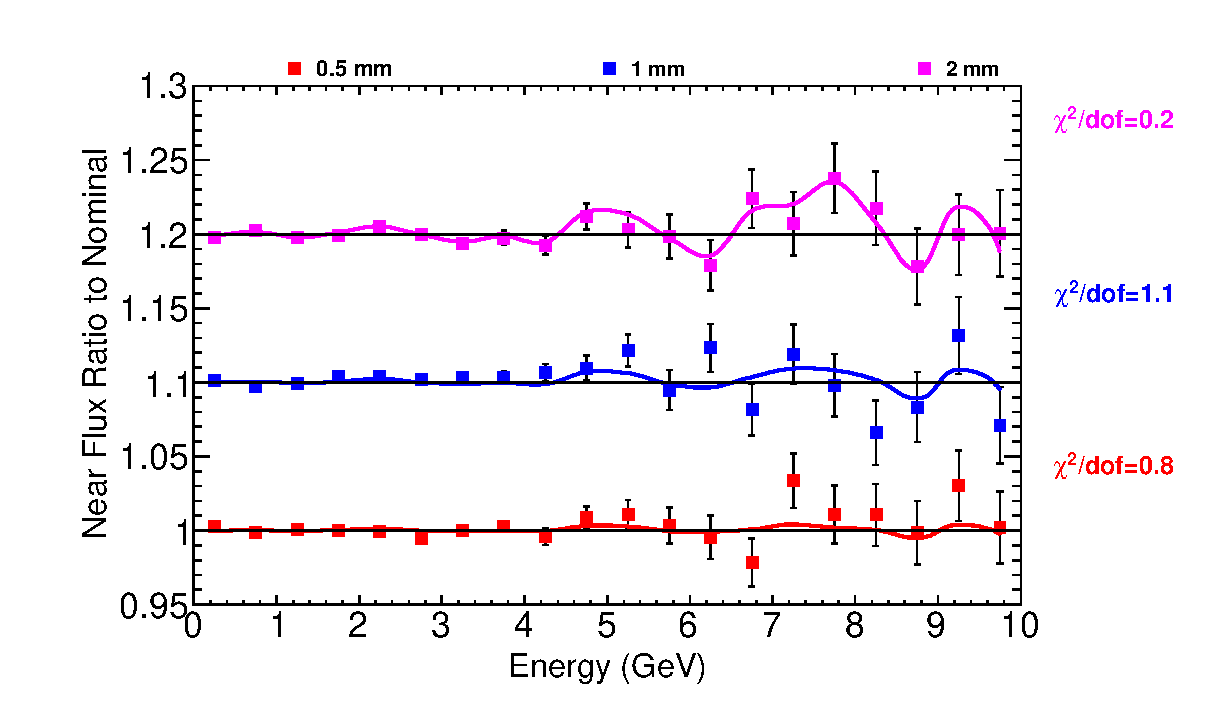
\includegraphics[width=6.0in]{figures/Horn2YTilt_near_summary.eps}}
  \end{center}
\caption{ Near detector flux ratios to nominal for several values of {\bf Horn 2 Tilt in $y$} (points) and the results of the fits to each energy bin (lines).}
\end{figure}

\begin{figure}[ht]
  \begin{center}
    {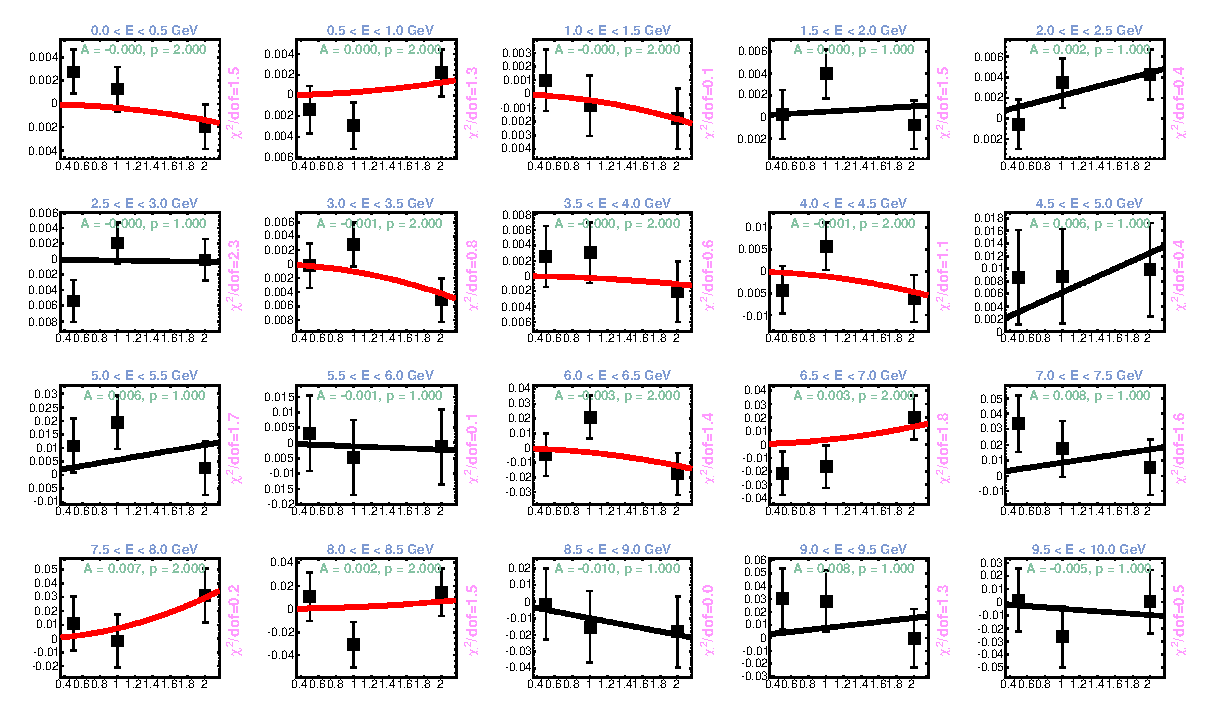
\includegraphics[width=5.0in]{figures/Horn2YTilt_near_fits.eps}}
  \end{center}
\caption{ Fits to the near flux ratios for several values of {\bf Horn 2 Tilt in $y$}. Black(Red) fit lines indicate that a linear(parabolic) fit provided the best $\chi^2$. }
\end{figure}

\begin{figure}[ht]
  \begin{center}
    {\includegraphics[width=6.0in]{figures/TargetXOffset_near_summary.eps}}
  \end{center}
\caption{ Near detector flux ratios to nominal for several values of {\bf Target Offset in $x$} (points) and the results of the fits to each energy bin (lines).}
\end{figure}

\begin{figure}[ht]
  \begin{center}
    {\includegraphics[width=5.0in]{figures/TargetXOffset_near_fits.eps}}
  \end{center}
\caption{ Fits to the near flux ratios for several values of {\bf Target Offset in $x$}. Black(Red) fit lines indicate that a linear(parabolic) fit provided the best $\chi^2$. }
\end{figure}

\begin{figure}[ht]
  \begin{center}
    {\includegraphics[width=6.0in]{figures/TargetYOffset_near_summary.eps}}
  \end{center}
\caption{ Near detector flux ratios to nominal for several values of {\bf Target Offset in $y$} (points) and the results of the fits to each energy bin (lines).}
\end{figure}

\begin{figure}[ht]
  \begin{center}
    {\includegraphics[width=5.0in]{figures/TargetYOffset_near_fits.eps}}
  \end{center}
\caption{ Fits to the near flux ratios for several values of {\bf Target Offset in $y$}. Black(Red) fit lines indicate that a linear(parabolic) fit provided the best $\chi^2$. }
\end{figure}

\begin{figure}[ht]
  \begin{center}
    {\includegraphics[width=6.0in]{figures/TargetXTilt_near_summary.eps}}
  \end{center}
\caption{ Near detector flux ratios to nominal for several values of {\bf Target Tilt in $x$} (points) and the results of the fits to each energy bin (lines).}
\end{figure}

\begin{figure}[ht]
  \begin{center}
    {\includegraphics[width=5.0in]{figures/TargetXTilt_near_fits.eps}}
  \end{center}
\caption{ Fits to the near flux ratios for several values of {\bf Target Tilt in $x$}. Black(Red) fit lines indicate that a linear(parabolic) fit provided the best $\chi^2$. }
\end{figure}

\clearpage

\begin{figure}[ht]
  \begin{center}
    {\includegraphics[width=6.0in]{figures/TargetYTilt_near_summary.eps}}
  \end{center}
\caption{ Near detector flux ratios to nominal for several values of {\bf Target Tilt in $y$} (points) and the results of the fits to each energy bin (lines).}
\end{figure}

\begin{figure}[ht]
  \begin{center}
    {\includegraphics[width=5.0in]{figures/TargetYTilt_near_fits.eps}}
  \end{center}
\caption{ Fits to the near flux ratios for several values of {\bf Target Tilt in $y$}. Black(Red) fit lines indicate that a linear(parabolic) fit provided the best $\chi^2$. }
\end{figure}


\begin{figure}[ht]
  \begin{center}
    {\includegraphics[width=6.0in]{figures/LBNEFDX_near_summary.eps}}
  \end{center}
\caption{ Near detector flux ratios to nominal for several values of {\bf Far detector offset in $x$} (points) and the results of the fits to each energy bin (lines).}
\end{figure}

\begin{figure}[ht]
  \begin{center}
    {\includegraphics[width=5.0in]{figures/LBNEFDX_near_fits.eps}}
  \end{center}
\caption{ Fits to the near flux ratios for several values of {\bf Far detector offset in $x$}. Black(Red) fit lines indicate that a linear(parabolic) fit provided the best $\chi^2$. }
\end{figure}

\begin{figure}[ht]
  \begin{center}
    {\includegraphics[width=6.0in]{figures/LBNEFDY_near_summary.eps}}
  \end{center}
\caption{ Near detector flux ratios to nominal for several values of {\bf Near detector offset in $y$} (points) and the results of the fits to each energy bin (lines).}
\end{figure}

\begin{figure}[ht]
  \begin{center}
    {\includegraphics[width=5.0in]{figures/LBNEFDY_near_fits.eps}}
  \end{center}
\caption{ Fits to the near flux ratios for several values of {\bf Near detector offset in $y$}. Black(Red) fit lines indicate that a linear(parabolic) fit provided the best $\chi^2$. }
\end{figure}

\begin{figure}[ht]
  \begin{center}
    {\includegraphics[width=6.0in]{figures/DecayPipeRadius_near_summary.eps}}
  \end{center}
\caption{ Near detector flux ratios to nominal for several values of {\bf Decay Pipe Radius} (points) and the results of the fits to each energy bin (lines).}
\end{figure}

\begin{figure}[ht]
  \begin{center}
    {\includegraphics[width=5.0in]{figures/DecayPipeRadius_near_fits.eps}}
  \end{center}
\caption{ Fits to the near flux ratios for several values of {\bf Decay Pipe Radius}. Black(Red) fit lines indicate that a linear(parabolic) fit provided the best $\chi^2$. }
\end{figure}

\begin{figure}[ht]
  \begin{center}
    {\includegraphics[width=6.0in]{figures/HornCurrent_near_summary.eps}}
  \end{center}
\caption{ Near detector flux ratios to nominal for several values of {\bf Horn Current} (points) and the results of the fits to each energy bin (lines).}
\end{figure}

\begin{figure}[ht]
  \begin{center}
    {\includegraphics[width=5.0in]{figures/HornCurrent_near_fits.eps}}
  \end{center}
\caption{ Fits to the near flux ratios for several values of {\bf HornCurrent}. Black(Red) fit lines indicate that a linear(parabolic) fit provided the best $\chi^2$. }
\end{figure}

\begin{figure}[ht]
  \begin{center}
    {\includegraphics[width=6.0in]{figures/BeamSigmaX_near_summary.eps}}
  \end{center}
\caption{ Near detector flux ratios to nominal for several values of {\bf Beam size in $x$} (points) and the results of the fits to each energy bin (lines).}
\end{figure}

\begin{figure}[ht]
  \begin{center}
    {\includegraphics[width=5.0in]{figures/BeamSigmaY_near_fits.eps}}
  \end{center}
\caption{ Fits to the near flux ratios for several values of {\bf Beam size in $y$}. Black(Red) fit lines indicate that a linear(parabolic) fit provided the best $\chi^2$. }
\end{figure}

\clearpage

\begin{figure}[ht]
  \begin{center}
    {\includegraphics[width=6.0in]{figures/Horn1XOffset_far_summary.eps}}
  \end{center}
\caption{ Far detector flux ratios to nominal for several values of {\bf Horn 1 Offset in $x$} (points) and the results of the fits to each energy bin (lines).}
\end{figure}

\begin{figure}[ht]
  \begin{center}
    {\includegraphics[width=5.0in]{figures/Horn1XOffset_far_fits.eps}}
  \end{center}
\caption{ Fits to the far flux ratios for several values of {\bf Horn 1 Offset in $x$}. Black(Red) fit lines indicate that a linear(parabolic) fit provided the best $\chi^2$. }
\end{figure}

\begin{figure}[ht]
  \begin{center}
    {\includegraphics[width=6.0in]{figures/Horn1YOffset_far_summary.eps}}
  \end{center}
\caption{ Far detector flux ratios to nominal for several values of {\bf Horn 1 Offset in $y$} (points) and the results of the fits to each energy bin (lines).}
\end{figure}

\begin{figure}[ht]
  \begin{center}
    {\includegraphics[width=5.0in]{figures/Horn1YOffset_far_fits.eps}}
  \end{center}
\caption{ Fits to the far flux ratios for several values of {\bf Horn 1 Offset in $y$}. Black(Red) fit lines indicate that a linear(parabolic) fit provided the best $\chi^2$. }
\end{figure}

\begin{figure}[ht]
  \begin{center}
    {\includegraphics[width=6.0in]{figures/Horn2XOffset_far_summary.eps}}
  \end{center}
\caption{ Far detector flux ratios to nominal for several values of {\bf Horn 2 Offset in $x$} (points) and the results of the fits to each energy bin (lines).}
\end{figure}

\begin{figure}[ht]
  \begin{center}
    {\includegraphics[width=5.0in]{figures/Horn2XOffset_far_fits.eps}}
  \end{center}
\caption{ Fits to the far flux ratios for several values of {\bf Horn 2 Offset in $x$}. Black(Red) fit lines indicate that a linear(parabolic) fit provided the best $\chi^2$. }
\end{figure}

\begin{figure}[ht]
  \begin{center}
    {\includegraphics[width=6.0in]{figures/Horn2YOffset_far_summary.eps}}
  \end{center}
\caption{ Far detector flux ratios to nominal for several values of {\bf Horn 2 Offset in $y$} (points) and the results of the fits to each energy bin (lines).}
\end{figure}

\begin{figure}[ht]
  \begin{center}
    {\includegraphics[width=5.0in]{figures/Horn2YOffset_far_fits.eps}}
  \end{center}
\caption{ Fits to the far flux ratios for several values of {\bf Horn 2 Offset in $y$}. Black(Red) fit lines indicate that a linear(parabolic) fit provided the best $\chi^2$. }
\end{figure}

\begin{figure}[ht]
  \begin{center}
    {\includegraphics[width=6.0in]{figures/Horn1XTilt_far_summary.eps}}
  \end{center}
\caption{ Far detector flux ratios to nominal for several values of {\bf Horn 1 Tilt in $x$} (points) and the results of the fits to each energy bin (lines).}
\end{figure}

\begin{figure}[ht]
  \begin{center}
    {\includegraphics[width=5.0in]{figures/Horn1XTilt_far_fits.eps}}
  \end{center}
\caption{ Fits to the far flux ratios for several values of {\bf Horn 1 Tilt in $x$}. Black(Red) fit lines indicate that a linear(parabolic) fit provided the best $\chi^2$. }
\end{figure}

\begin{figure}[ht]
  \begin{center}
    {\includegraphics[width=6.0in]{figures/Horn1YTilt_far_summary.eps}}
  \end{center}
\caption{ Far detector flux ratios to nominal for several values of {\bf Horn 1 Tilt in $y$} (points) and the results of the fits to each energy bin (lines).}
\end{figure}

\begin{figure}[ht]
  \begin{center}
    {\includegraphics[width=5.0in]{figures/Horn1YTilt_far_fits.eps}}
  \end{center}
\caption{ Fits to the far flux ratios for several values of {\bf Horn 1 Tilt in $y$}. Black(Red) fit lines indicate that a linear(parabolic) fit provided the best $\chi^2$. }
\end{figure}

\clearpage

\begin{figure}[ht]
  \begin{center}
    {\includegraphics[width=6.0in]{figures/Horn2XTilt_far_summary.eps}}
  \end{center}
\caption{ Far detector flux ratios to nominal for several values of {\bf Horn 2 Tilt in $x$} (points) and the results of the fits to each energy bin (lines).}
\end{figure}

\begin{figure}[ht]
  \begin{center}
    {\includegraphics[width=5.0in]{figures/Horn2XTilt_far_fits.eps}}
  \end{center}
\caption{ Fits to the far flux ratios for several values of {\bf Horn 2 Tilt in $x$}. Black(Red) fit lines indicate that a linear(parabolic) fit provided the best $\chi^2$. }
\end{figure}

\begin{figure}[ht]
  \begin{center}
    {\includegraphics[width=6.0in]{figures/Horn2YTilt_far_summary.eps}}
  \end{center}
\caption{ Far detector flux ratios to nominal for several values of {\bf Horn 2 Tilt in $y$} (points) and the results of the fits to each energy bin (lines).}
\end{figure}

\begin{figure}[ht]
  \begin{center}
    {\includegraphics[width=5.0in]{figures/Horn2YTilt_far_fits.eps}}
  \end{center}
\caption{ Fits to the far flux ratios for several values of {\bf Horn 2 Tilt in $y$}. Black(Red) fit lines indicate that a linear(parabolic) fit provided the best $\chi^2$. }
\end{figure}

\begin{figure}[ht]
  \begin{center}
    {\includegraphics[width=6.0in]{figures/TargetXOffset_far_summary.eps}}
  \end{center}
\caption{ Far detector flux ratios to nominal for several values of {\bf Target Offset in $x$} (points) and the results of the fits to each energy bin (lines).}
\end{figure}

\begin{figure}[ht]
  \begin{center}
    {\includegraphics[width=5.0in]{figures/TargetXOffset_far_fits.eps}}
  \end{center}
\caption{ Fits to the far flux ratios for several values of {\bf Target Offset in $x$}. Black(Red) fit lines indicate that a linear(parabolic) fit provided the best $\chi^2$. }
\end{figure}

\begin{figure}[ht]
  \begin{center}
    {\includegraphics[width=6.0in]{figures/TargetYOffset_far_summary.eps}}
  \end{center}
\caption{ Far detector flux ratios to nominal for several values of {\bf Target Offset in $y$} (points) and the results of the fits to each energy bin (lines).}
\end{figure}

\begin{figure}[ht]
  \begin{center}
    {\includegraphics[width=5.0in]{figures/TargetYOffset_far_fits.eps}}
  \end{center}
\caption{ Fits to the far flux ratios for several values of {\bf Target Offset in $y$}. Black(Red) fit lines indicate that a linear(parabolic) fit provided the best $\chi^2$. }
\end{figure}

\begin{figure}[ht]
  \begin{center}
    {\includegraphics[width=6.0in]{figures/TargetXTilt_far_summary.eps}}
  \end{center}
\caption{ Far detector flux ratios to nominal for several values of {\bf Target Tilt in $x$} (points) and the results of the fits to each energy bin (lines).}
\end{figure}

\begin{figure}[ht]
  \begin{center}
    {\includegraphics[width=5.0in]{figures/TargetXTilt_far_fits.eps}}
  \end{center}
\caption{ Fits to the far flux ratios for several values of {\bf Target Tilt in $x$}. Black(Red) fit lines indicate that a linear(parabolic) fit provided the best $\chi^2$. }
\end{figure}

\clearpage

\begin{figure}[ht]
  \begin{center}
    {\includegraphics[width=6.0in]{figures/TargetYTilt_far_summary.eps}}
  \end{center}
\caption{ Far detector flux ratios to nominal for several values of {\bf Target Tilt in $y$} (points) and the results of the fits to each energy bin (lines).}
\end{figure}

\begin{figure}[ht]
  \begin{center}
    {\includegraphics[width=5.0in]{figures/TargetYTilt_far_fits.eps}}
  \end{center}
\caption{ Fits to the far flux ratios for several values of {\bf Target Tilt in $y$}. Black(Red) fit lines indicate that a linear(parabolic) fit provided the best $\chi^2$. }
\end{figure}


\begin{figure}[ht]
  \begin{center}
    {\includegraphics[width=6.0in]{figures/LBNEFDX_far_summary.eps}}
  \end{center}
\caption{ Far detector flux ratios to nominal for several values of {\bf Far detector offset in $x$} (points) and the results of the fits to each energy bin (lines).}
\end{figure}

\begin{figure}[ht]
  \begin{center}
    {\includegraphics[width=5.0in]{figures/LBNEFDX_far_fits.eps}}
  \end{center}
\caption{ Fits to the far flux ratios for several values of {\bf Far detector offset in $x$}. Black(Red) fit lines indicate that a linear(parabolic) fit provided the best $\chi^2$. }
\end{figure}

\begin{figure}[ht]
  \begin{center}
    {\includegraphics[width=6.0in]{figures/LBNEFDY_far_summary.eps}}
  \end{center}
\caption{ Far detector flux ratios to nominal for several values of {\bf Far detector offset in $y$} (points) and the results of the fits to each energy bin (lines).}
\end{figure}

\begin{figure}[ht]
  \begin{center}
    {\includegraphics[width=5.0in]{figures/LBNEFDY_far_fits.eps}}
  \end{center}
\caption{ Fits to the far flux ratios for several values of {\bf Far detector offset in $y$}. Black(Red) fit lines indicate that a linear(parabolic) fit provided the best $\chi^2$. }
\end{figure}

\begin{figure}[ht]
  \begin{center}
    {\includegraphics[width=6.0in]{figures/DecayPipeRadius_far_summary.eps}}
  \end{center}
\caption{ Far detector flux ratios to nominal for several values of {\bf Decay Pipe Radius} (points) and the results of the fits to each energy bin (lines).}
\end{figure}

\begin{figure}[ht]
  \begin{center}
    {\includegraphics[width=5.0in]{figures/DecayPipeRadius_far_fits.eps}}
  \end{center}
\caption{ Fits to the far flux ratios for several values of {\bf Decay Pipe Radius}. Black(Red) fit lines indicate that a linear(parabolic) fit provided the best $\chi^2$. }
\end{figure}

\begin{figure}[ht]
  \begin{center}
    {\includegraphics[width=6.0in]{figures/HornCurrent_far_summary.eps}}
  \end{center}
\caption{ Far detector flux ratios to nominal for several values of {\bf Horn Current} (points) and the results of the fits to each energy bin (lines).}
\end{figure}

\begin{figure}[ht]
  \begin{center}
    {\includegraphics[width=5.0in]{figures/HornCurrent_far_fits.eps}}
  \end{center}
\caption{ Fits to the far flux ratios for several values of {\bf HornCurrent}. Black(Red) fit lines indicate that a linear(parabolic) fit provided the best $\chi^2$. }
\end{figure}

\begin{figure}[ht]
  \begin{center}
    {\includegraphics[width=6.0in]{figures/BeamSigmaX_far_summary.eps}}
  \end{center}
\caption{ Far detector flux ratios to nominal for several values of {\bf Beam size in $x$} (points) and the results of the fits to each energy bin (lines).}
\end{figure}

\begin{figure}[ht]
  \begin{center}
    {\includegraphics[width=5.0in]{figures/BeamSigmaY_far_fits.eps}}
  \end{center}
\caption{ Fits to the far flux ratios for several values of {\bf Beam size in $y$}. Black(Red) fit lines indicate that a linear(parabolic) fit provided the best $\chi^2$. }
\end{figure}

\begin{figure}[ht]
  \begin{center}
    {\includegraphics[width=6.0in]{figures/tot_error_nof.eps}}
  \end{center}
\caption{ Total fractional alignment systematic uncertainty as a function of energy on the near/far flux ratio. }
\end{figure}

\begin{figure}[ht]
  \begin{center}
    {\includegraphics[width=6.0in]{figures/tot_error_near.eps}}
  \end{center}
\caption{ Total fractional alignment systematic uncertainty as a function of energy on the flux at the near detector. }
\end{figure}

\begin{figure}[ht]
  \begin{center}
    {\includegraphics[width=6.0in]{figures/tot_error_far.eps}}
  \end{center}
\caption{ Total fractional alignment systematic uncertainty as a function of energy on the flux at the far detector. }
\end{figure}

\begin{figure}[ht]
  \begin{center}
    {\includegraphics[width=6.0in]{figures/error_summary_nof.eps}}
  \end{center}
\caption{ Summary of alignment systematic uncertainties on the near/far flux ratio.}
\end{figure}

\begin{figure}[ht]
  \begin{center}
    {\includegraphics[width=6.0in]{figures/error_summary_near.eps}}
  \end{center}
\caption{ Summary of alignment systematic uncertainties on the flux at the near detector.}
\end{figure}

\begin{figure}[ht]
  \begin{center}
    {\includegraphics[width=6.0in]{figures/error_summary_far.eps}}
  \end{center}
\caption{ Summary of alignment systematic uncertainties on the flux at the far detector.}
\end{figure}



\begin{thebibliography}{1}

%\cite{Barlow:1993dm}
\bibitem{Barlow:1993dm} 
  R.~J.~Barlow and C.~Beeston,
  %``Fitting using finite Monte Carlo samples,''
  Comput.\ Phys.\ Commun.\  {\bf 77}, 219 (1993).
  %%CITATION = CPHCB,77,219;%%
  
\end{thebibliography}


\end{document}

























